%!TEX root = ../thesis.tex
%*******************************************************************************
%****************************** Third Chapter **********************************
%*******************************************************************************
\chapter{Results and Discussion}
\label{chap:results}
% **************************** Define Graphics Path **************************
\ifpdf
    \graphicspath{{Chapter3/Figs/Raster/}{Chapter3/Figs/PDF/}{Chapter3/Figs/}}
\else
    \graphicspath{{Chapter3/Figs/Vector/}{Chapter3/Figs/}}
\fi

In this chapter we present the performance of the classifiers under the different split schemes outlined earlier. The various features used and their applicability on different splitting conditions is also be evaluated. 

The confusion matrix used has the form 
\begin{align}
	\begin{bmatrix}
	\text{True Black/ Black Predicted correctly}&\text{False White/ Black  Predicted falsely}\\
	\text{False Black/ White Predicted falsely}&\text{True White/ White  Predicted correctly}
	\end{bmatrix}
\end{align}



The results of the benchmark method we devised in section \ref{sec:splitting} are presented in table \ref{table:benchmarksim} for maximum similarity, table \ref{table:benchmarkdissim} for maximum dissimilarity, and table \ref{table:benchmarkrand} for random splits. The two row names differentiate between the set of response variables used for the benchmark's evaluation; All Labels indicates the use of all the river samples, Min Labels of those whose total OTU read-count is more than 10000. The accuracy is also included in a separate row so as to make comparisons between methods easier. A quick glance shows that the benchmark has a much lower accuracy than the class prior of the data set (87.2\%), as was suggested in section \ref{sec:splitting}.



\begin{table}
	\centering
		\caption{Benchmark for Maximum Similarity}
	\label{table:benchmarksim}
	\begin{tabular}{l c c c}
		\toprule 
		&\multicolumn{2}{c}{Confusion Matrix} &Accuracy\\
		Features used & Predicted Black&Predicted White&\\ 
		
		\midrule
		\multirow{2}{*}{All Labels }& 	2.64 & 18.36&		\multirow{2}{*}{77.6\%}\\
					&	18.36 &124.64&\\
		\cmidrule{2-3}
		\multirow{2}{*}{Min Labels}  &2.75 & 18.25&		\multirow{2}{*}{76.8\%}\\
		&18.25& 117.75&\\
		\bottomrule

	\end{tabular}

\end{table}

\begin{table}[!h]
	\centering
		\caption{Benchmark for Maximum Dissimilarity}
	\label{table:benchmarkdissim}
	\begin{tabular}{l c c c }
		\toprule 
		&\multicolumn{2}{c}{Confusion Matrix} & Accuracy\\
		Features used & Predicted Black&Predicted White&\\ 
		
		\midrule
		\multirow{2}{*}{All Labels }&  1.75 &19.25&\multirow{2}{*}{76.7\%}\\
								  &	 18.96&124.04 &\\
		\cmidrule{2-3}
		\multirow{2}{*}{Min Labels}    &1.83&19.17&\multirow{2}{*}{75.8\% }\\
									&18.83&117.17&\\
		\bottomrule

	\end{tabular}

\end{table}

%RANDOM SPLITS
\begin{table}[!h]
	\centering
		\caption{Benchmark for Maximum Dissimilarity}
	\label{table:benchmarkrand}
	\begin{tabular}{l c c c }
		\toprule 
		&\multicolumn{2}{c}{Confusion Matrix} & Accuracy\\
		Features used & Predicted Black&Predicted White&\\ 
		
		\midrule
		\multirow{2}{*}{All Labels }& 2.69 &18.31&\multirow{2}{*}{77.7\%}\\
		&	 18.31&124.69 &\\
		\cmidrule{2-3}
		\multirow{2}{*}{Min Labels}    &2.81&18.19&\multirow{2}{*}{76.8\% }\\
		&18.19&117.81&\\
		\bottomrule
	\end{tabular}

\end{table}
%%%
%
%SIMILARITY
\section{Maximum Similarity}
The results for Logistic regression and Random forest tested on the maximum similarity scheme are shown in tables \ref{table:lrdissimilarity} and \ref{table:rfrsimilarity} respectively. Both methods performed relatively well when compared to the baseline. Furthermore, the PCoA features produced poorer results than the OTU ones. This was also the case when fewer dimensions, describing 99\% and 90\% of the variance, were chosen as features. The results for these can be found in the appendix in tables \ref{table:lrdissimilarityappendix} and \ref{table:rfrsimilarityappendix}. The results for a 20-dimensional NMDS configuration were also included there and not in this Chapter because the method failed to converge to a minimum stress.

Using the F score to find the best model in the cross validation step resulted in a lower number of black water samples correctly identified. This was especially the case of Random Forest. Therefore, we present the performance of the models selected using accuracy.

Just from the accuracy score we can see that Logistic regression outperforms Random Forests. The best score for the former is 98.78\% using OTU LOW and close second is 98.17\% using OTU, OTU CSS, and OTU CSS LOG. For Random Forests, OTU CSS LOG has the best score of 96.95\% and close second is OTU CSS and OTU LOW with 96.34\%. Both methods have significantly better results than the baseline's 77.6\% and 76.8\% accuracy (the second is used to compare the OTU MIN CSS set).

It also interesting that Random Forest has an equal or lower Recall for Black water samples for all feature sets. In other words, given that a sample comes from black waters, the classifier predicts it as such with a lower probability than Logistic regression. 

Using the $L_1$ penalty in Logistic regression has reduced the coefficients of many features to zero. From the best performing sets, the percentage of zero coefficients to the total number is 82.34\% (OTU LOW), 85.29\% (OTU), 88.95\% (OTU CSS), and 95.32\% (OTU CSS LOG). From the remaining species, 3.79\% of them have non zero coefficients in three sets (OTU CSS< OTU CSS LOG, and OTU). This means that there are only a limited number of informative species that help us identify the water colour. 


%LOGISTIC SIM
\begin{table}[!h]
\centering
\caption{Results from maximising similarity using Logistic Regression}
\label{table:lrsimilarity}
\begin{tabular}{l c  c c}
\toprule
		&\multicolumn{2}{c}{Confusion Matrix} & Accuracy\\
Features used & Predicted Black&Predicted White&\\
\midrule
\multirow{2}{*}{OTU} &19 &2&\multirow{2}{*}{98.17\%}\\
&	 1&142&\\
\cmidrule{2-3}
\multirow{2}{*}{OTU LOW} &19 &2&\multirow{2}{*}{98.78\%}\\
&	 0&143&\\
\cmidrule{2-3}
\multirow{2}{*}{OTU CSS}&18 &3&\multirow{2}{*}{98.17\%}\\
&	 0&143&\\
\cmidrule{2-3}
\multirow{2}{*}{OTU Min CSS}&18 &3&\multirow{2}{*}{98.09\%}\\
&	 0&136&\\
\cmidrule{2-3}
\multirow{2}{*}{OTU CSS LOG}&19 &2&\multirow{2}{*}{98.17\%}\\
&	 1&142&\\
\cmidrule{2-3}
\multirow{2}{*}{PCoA Bray-Curtis} &16 &5&\multirow{2}{*}{95.12\%}\\
&	 3&140&\\
\cmidrule{2-3}
\multirow{2}{*}{PCoA Bray-Curtis CSS} &16 &5&\multirow{2}{*}{96.34\%}\\
&	 1&142&\\
\bottomrule
\end{tabular}

\end{table}


% RFR similarirtty
\begin{table}[!h]
	\centering
	\caption{Results from maximising similarity using Random Forest}
	\label{table:rfrsimilarity}
\begin{tabular}{l c  c c}
	\toprule
	&\multicolumn{2}{c}{Confusion Matrix} & Accuracy\\
	Features used & Predicted Black&Predicted White&\\
	
	\midrule
	\multirow{2}{*}{OTU} &17 &4&\multirow{2}{*}{95.73\%}\\
	&	 3&140&\\
	\cmidrule{2-3}
	\multirow{2}{*}{OTU LOW} &18 &3&\multirow{2}{*}{96.34\%}\\
	&	 3&140&\\
	\cmidrule{2-3}
	\multirow{2}{*}{OTU CSS} &18 &3&\multirow{2}{*}{96.34\%}\\
	&	 3&140&\\
	\cmidrule{2-3}
	\multirow{2}{*}{OTU Min CSS}&18 &3&\multirow{2}{*}{96.18\%}\\
	&	 3&133&\\
	\cmidrule{2-3}
	\multirow{2}{*}{OTU CSS LOG} &19 &2&\multirow{2}{*}{96.95\%}\\
	&	 3&140&\\
	\cmidrule{2-3}
	\multirow{2}{*}{PCoA Bray-Curtis} &6 &15&\multirow{2}{*}{88.41\%}\\
	&	 4&139&\\
	\cmidrule{2-3}
	\multirow{2}{*}{PCoA Bray-Curtis CSS} &4 &17&\multirow{2}{*}{89.63\%}\\
	&	 0&143&\\
	\bottomrule
\end{tabular}

\end{table}

To explore which of these species contribute most to classification we used the feature importance of Random Forests. However, instead of checking only for individual species' predictive ability, we used the taxonomic order as an aggregating factor, to get a sense which contributes the most. This was done by averaging the importance of each species, as reported by Random Forests, within their Order. The results are presented for some feature sets in the form of pie charts in Figures \ref{fig:simmeanotucss} and \ref{fig:simmeanotucsslog}. For other features were this evaluation of taxonomic importance was possible are presented in the Appendix, in Figures \ref{fig:simotumean} and \ref{fig:simotumincssmean}. 

For all feature sets used, species in the \textit{Perissodactyla} Order have on average the most explanatory power. However, this Order is only composed of two (sub)species; the South American and Mountain tapir. This method of aggregating feature importance thus favours orders with few species. It is evident in the next most important taxonomic Order as well, the \textit{Cetacea}, which is again composed of two species; the Amazon river dolphin (which is technically a whale) and Tucuxi (a freshwater dolphin). 

Therefore, another aggregating method has to be used to get a better idea of the explanatory power of the whole taxonomic Order. We chose to do this by summing the importance of each species, within their Order. The results are shown in Figures \ref{fig:simsumotucss} and \ref{fig:simsumotucsslog} (\ref{fig:simotusum} and \ref{fig:simotumincsssum} in the Appendix), and highlight different Orders. In particular, \textit{Characiformes} and \textit{Siluriformes} are in sum the most explanatory ones. This is to be expected however, since they are the most populous as well (although in reverse order) and summing importance will inevitably favour the most numerous groups. 



\begin{figure}[!h]
	\centering

	\begin{subfigure}{0.45\textwidth}
	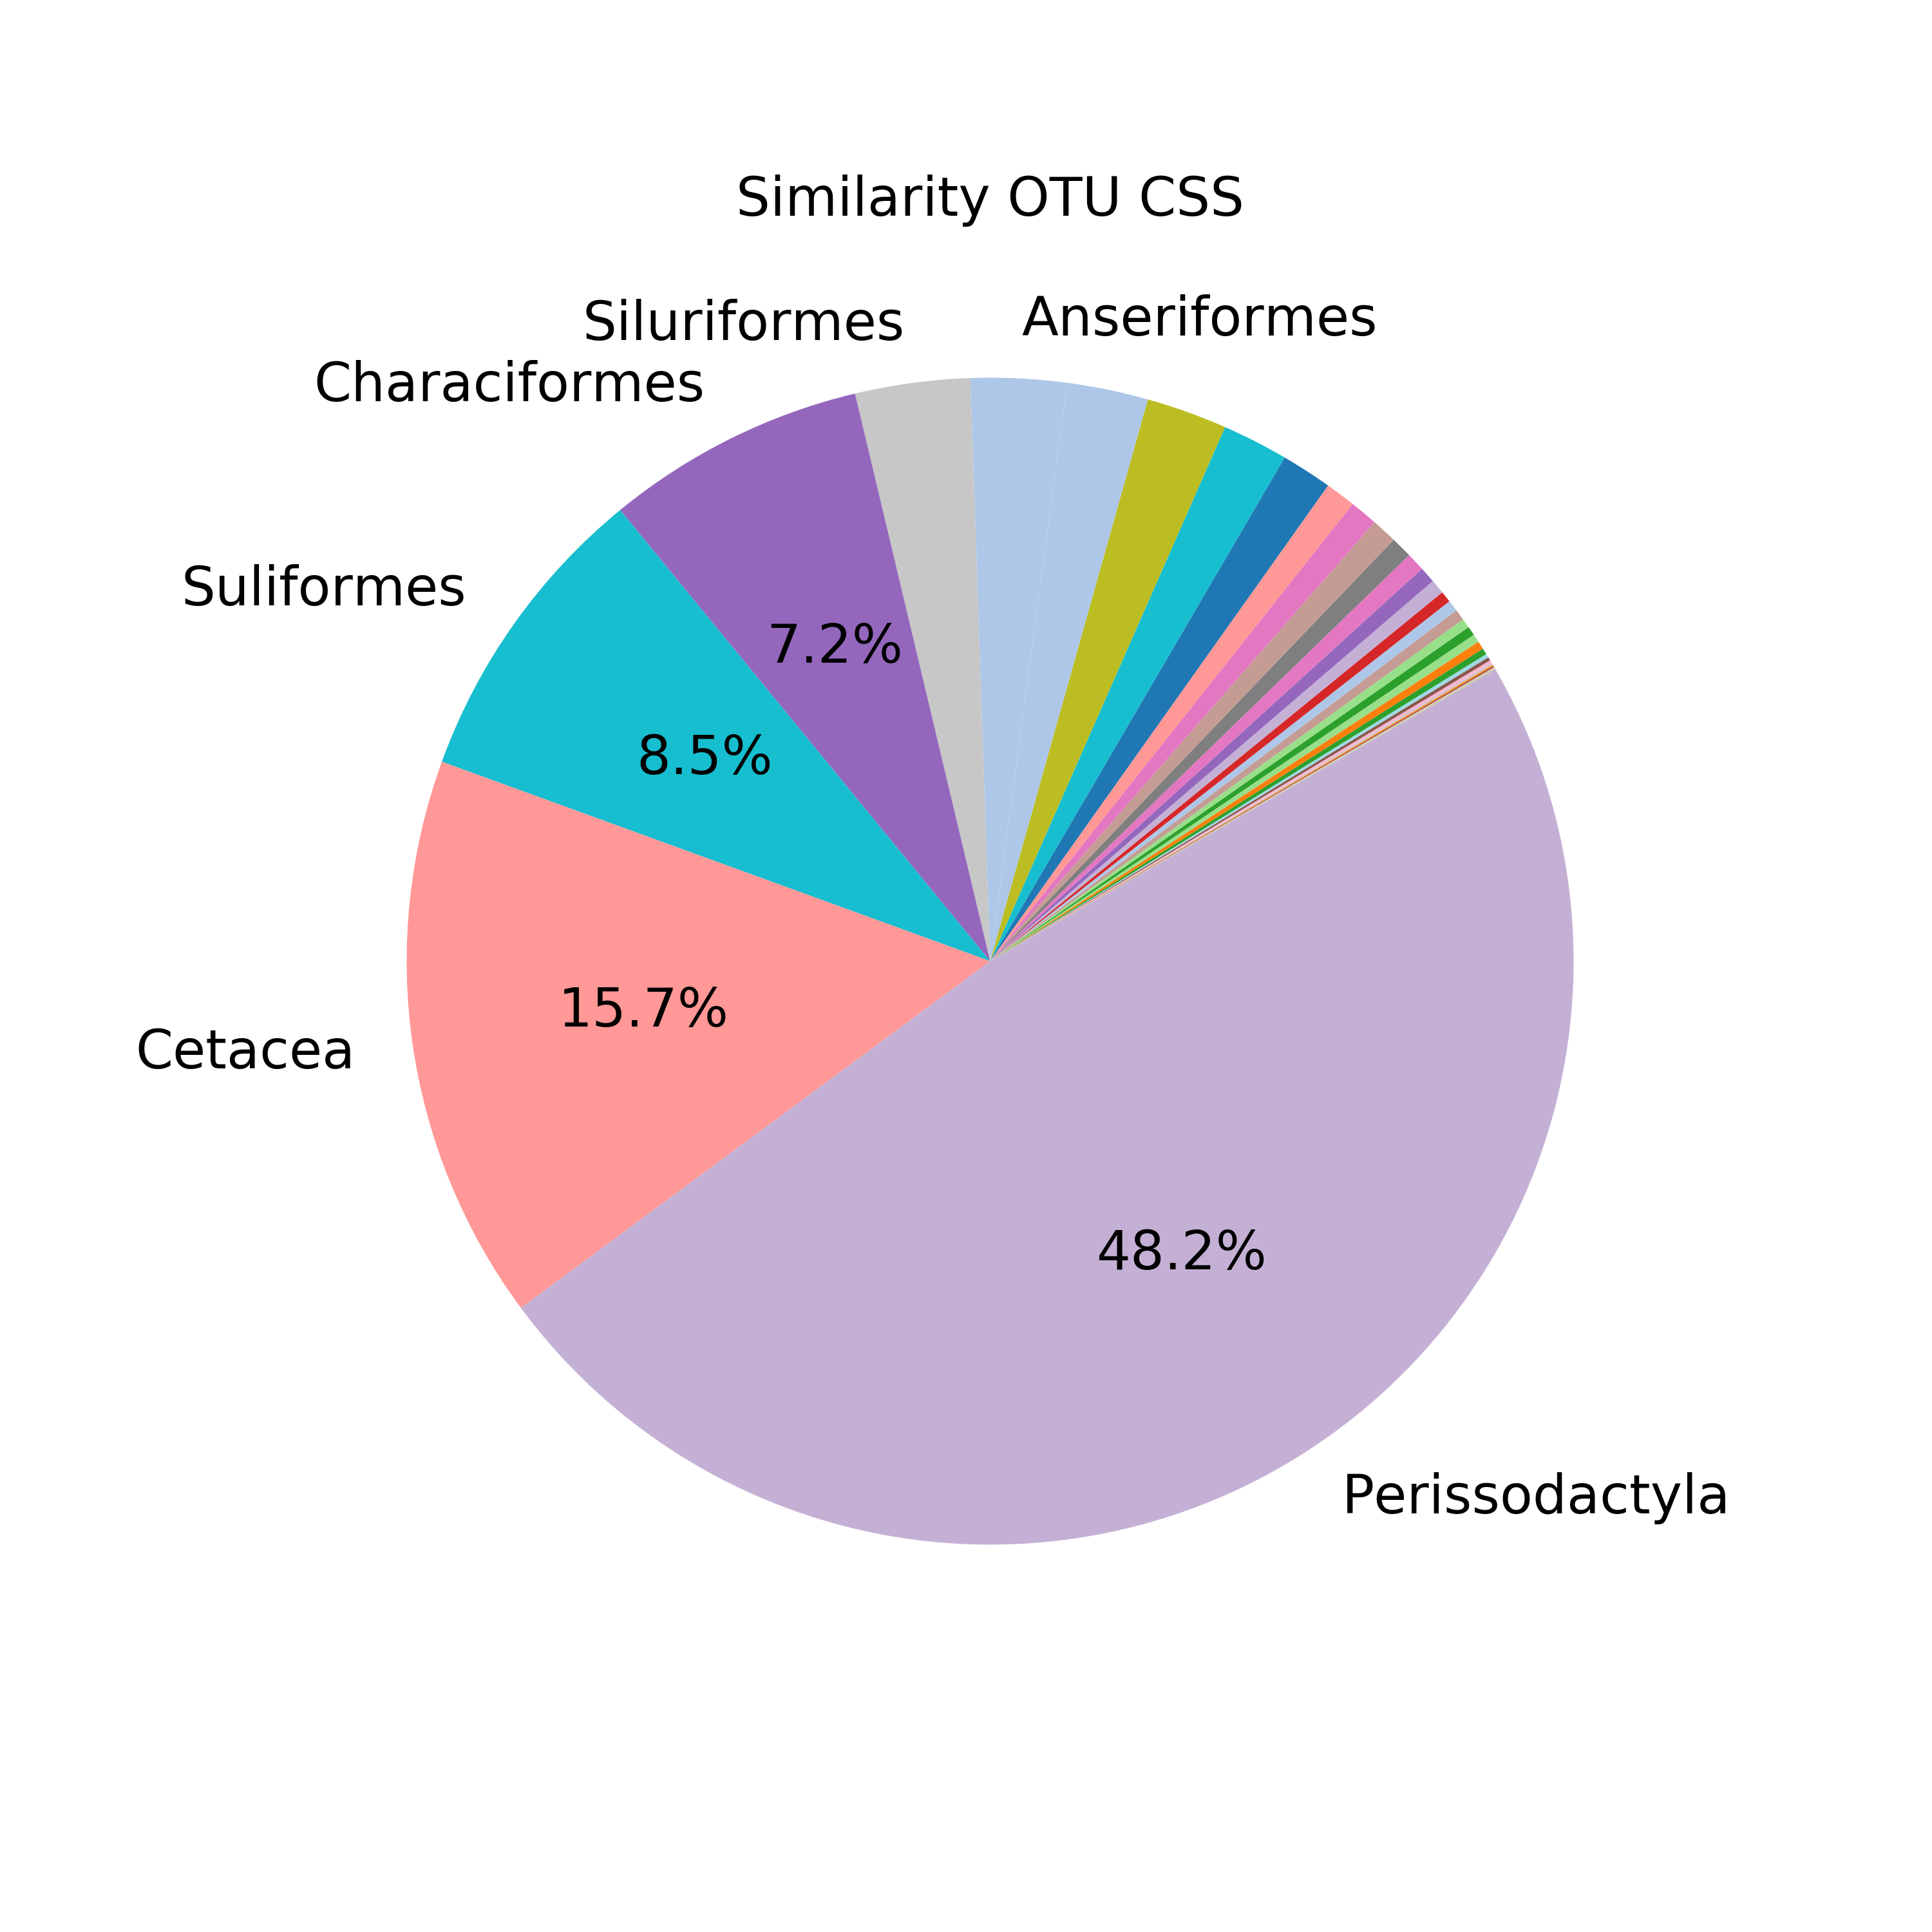
\includegraphics[width=\textwidth]{rfr_sim_mean_pieOTU CSS}
	\caption{}
	\label{fig:simmeanotucss}
	\end{subfigure}	
	\begin{subfigure}{0.45\textwidth}
		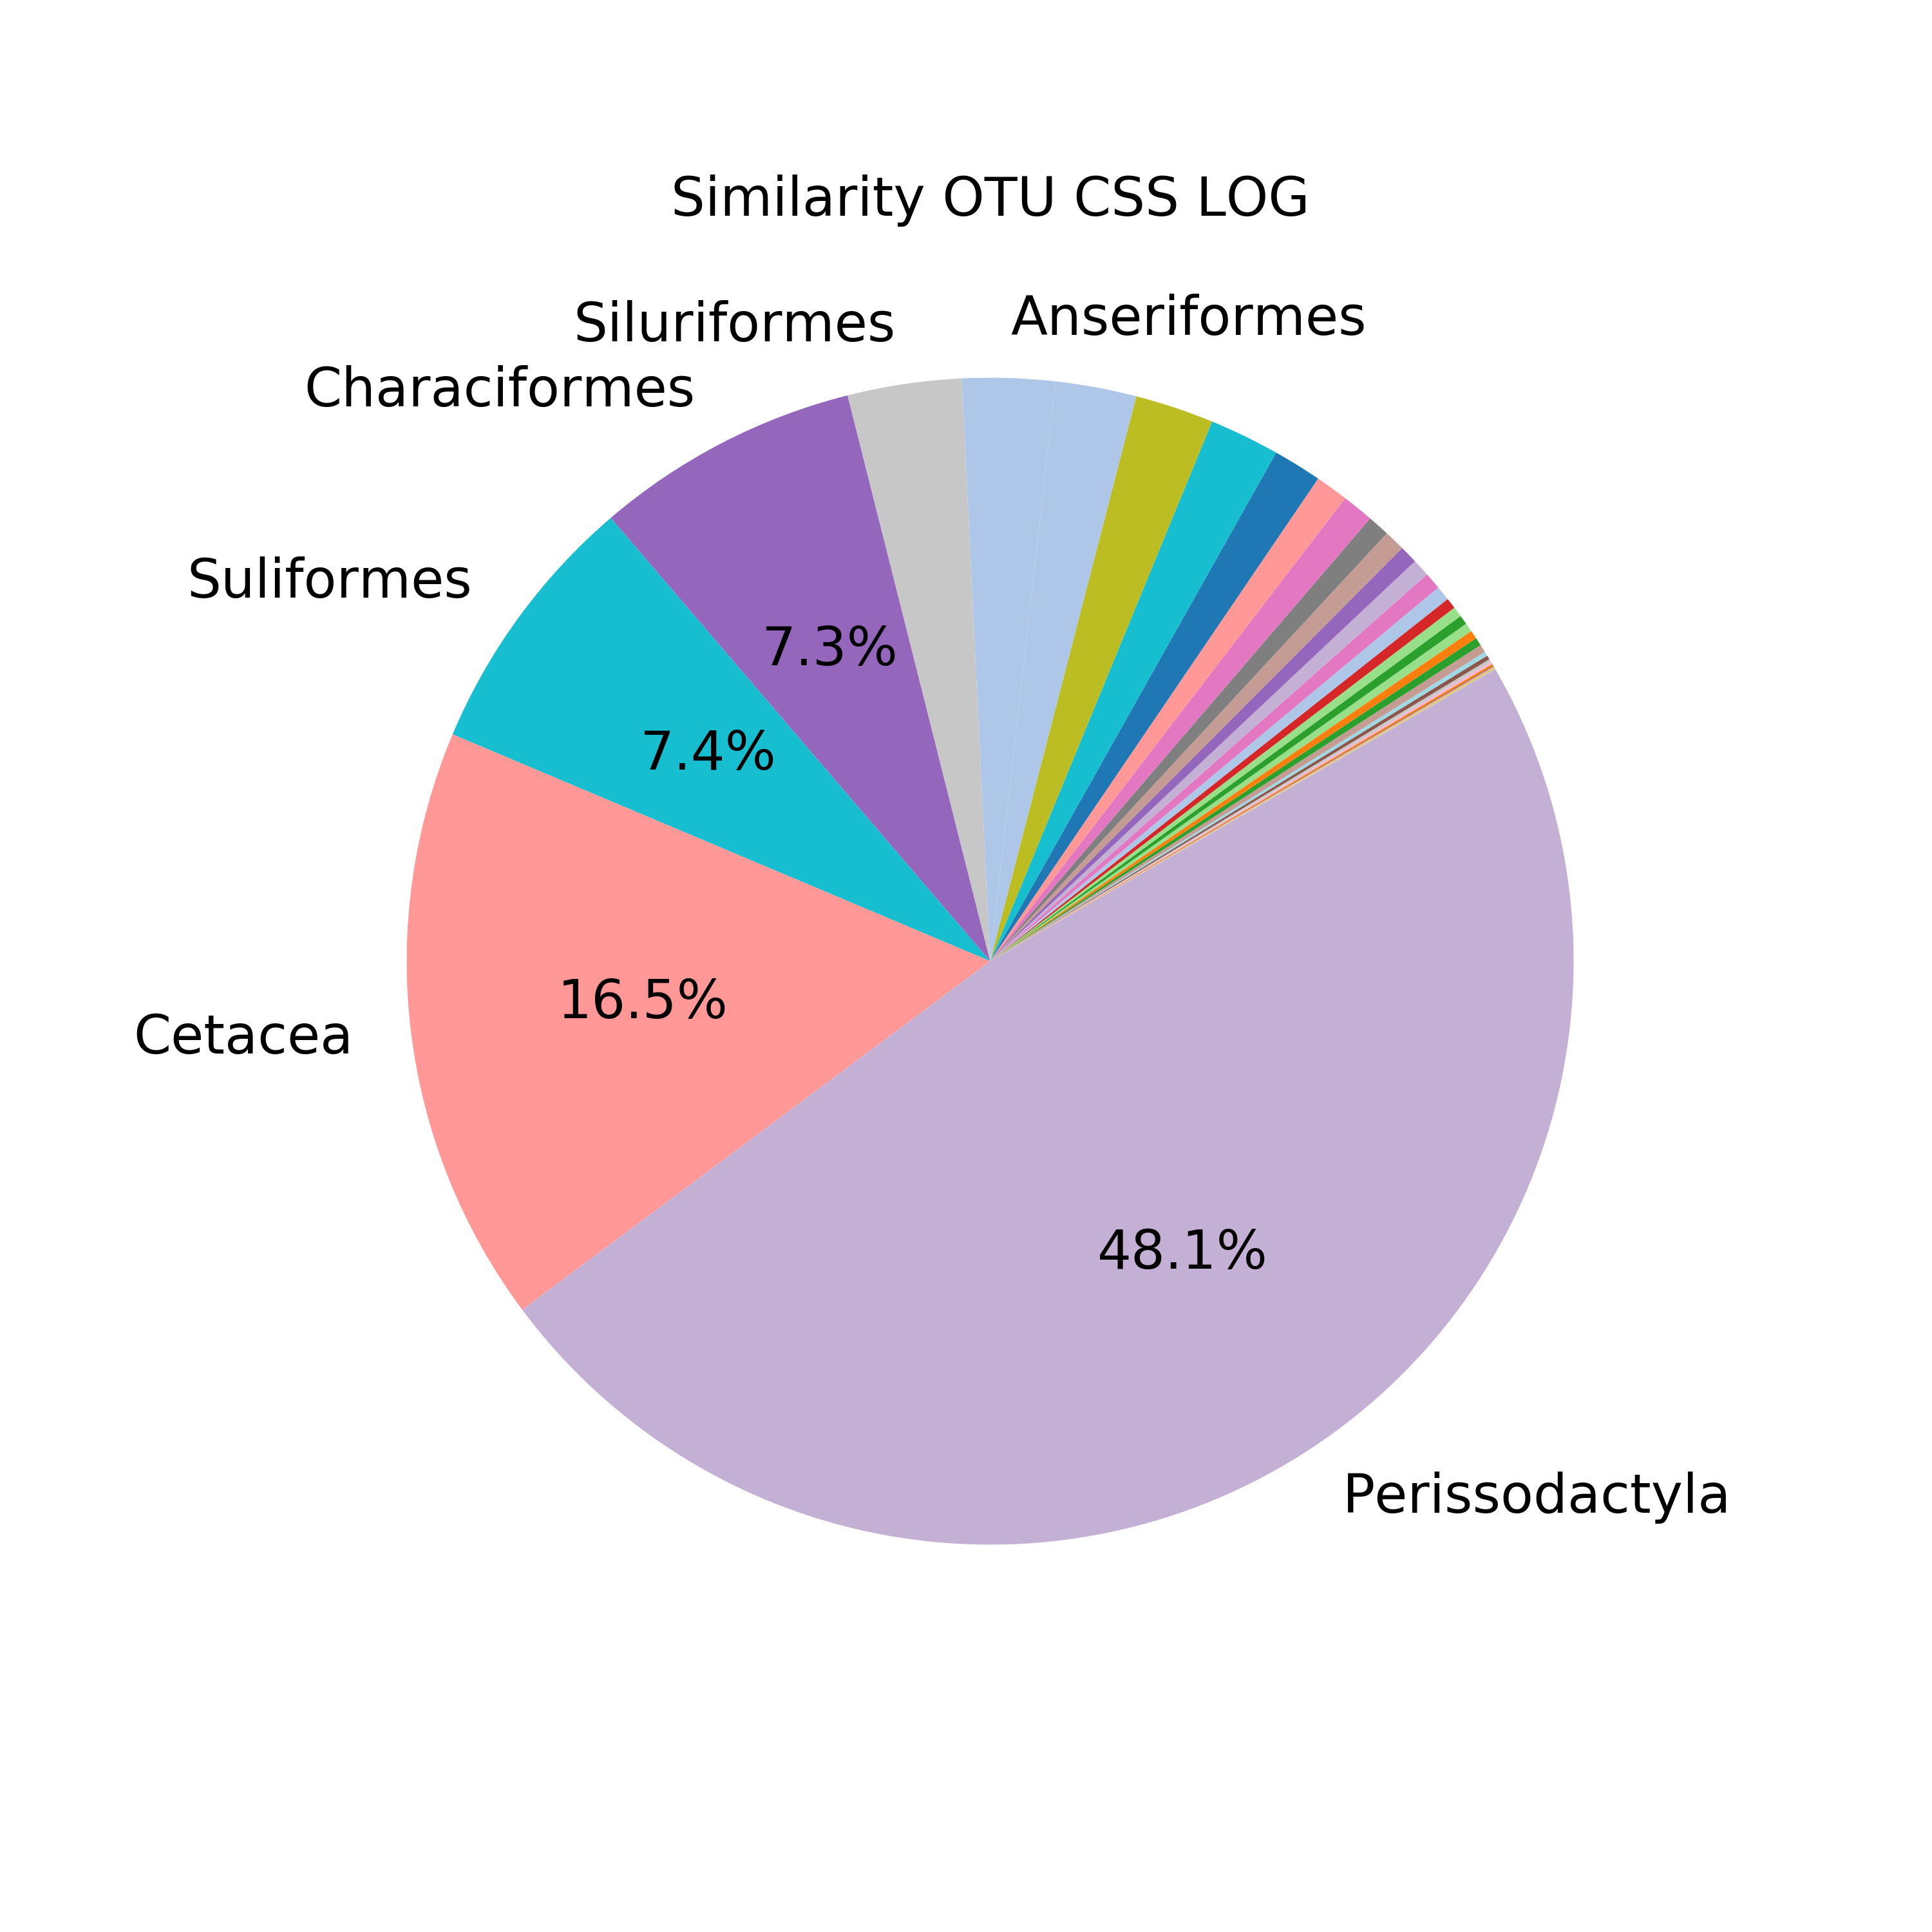
\includegraphics[width=\textwidth]{rfr_sim_mean_pieOTU CSS LOG}
		\caption{}
		\label{fig:simmeanotucsslog}
	\end{subfigure}\\
	\begin{subfigure}{0.45\textwidth}
	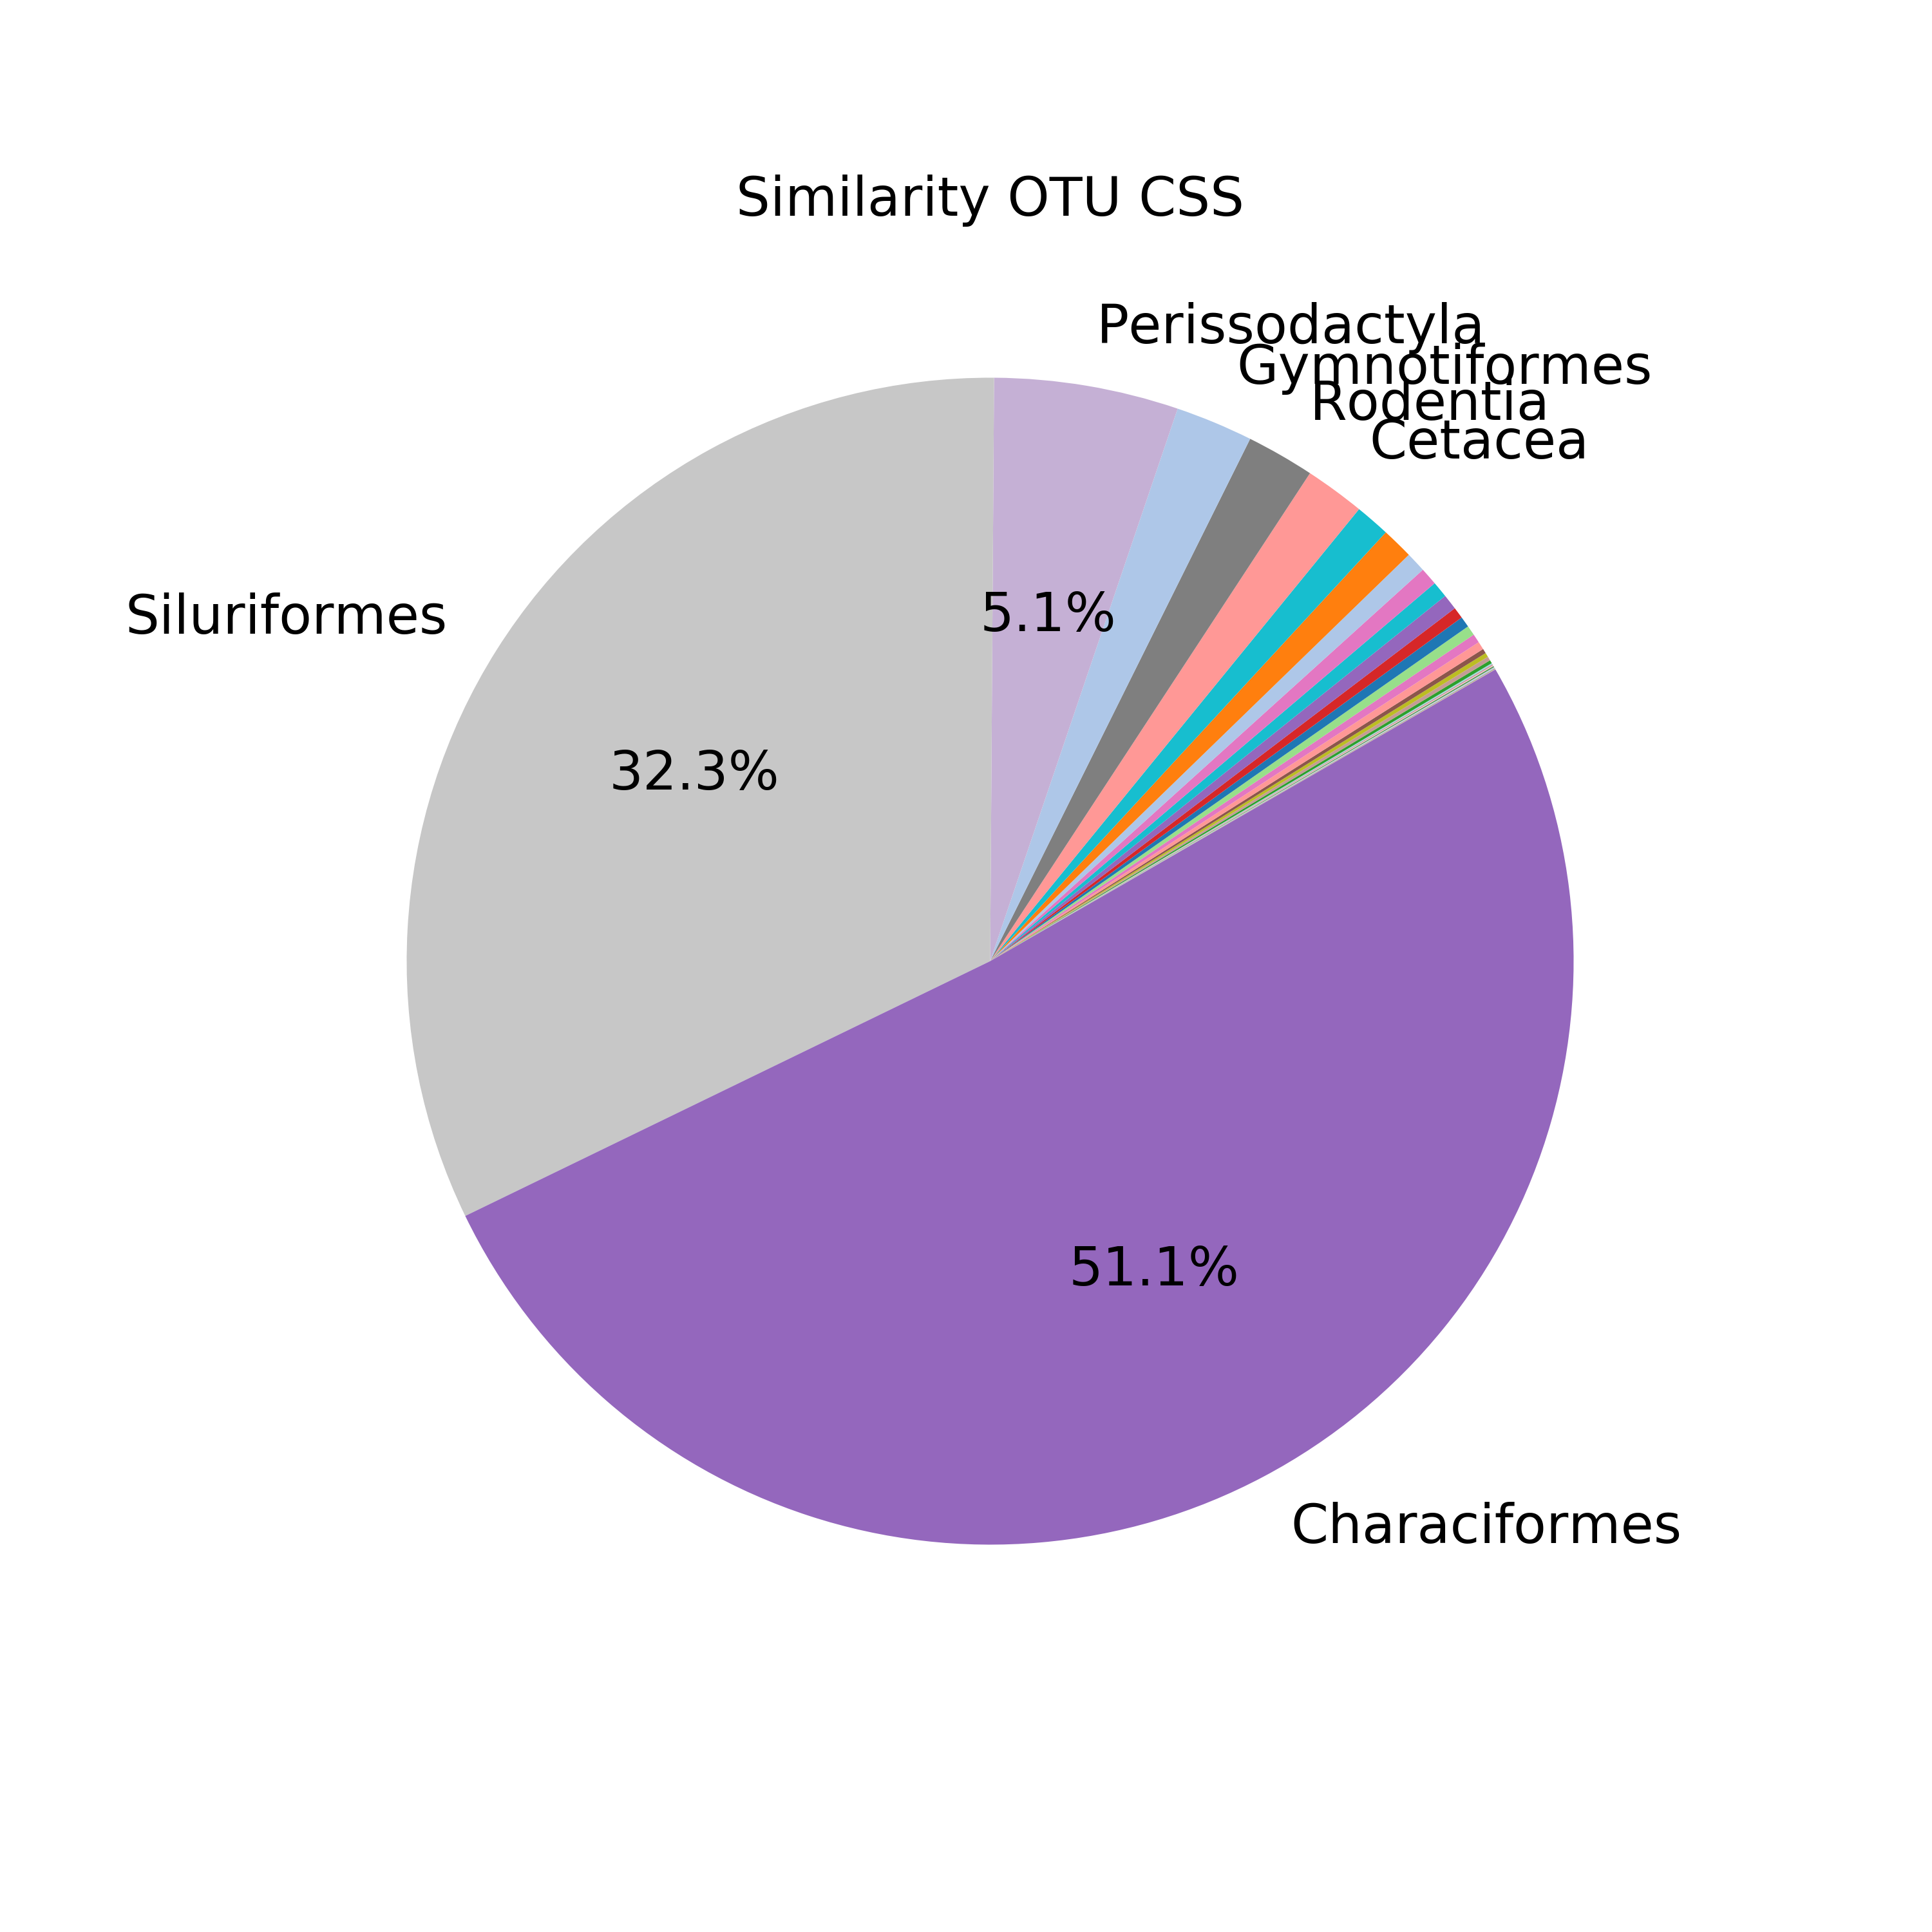
\includegraphics[width=\textwidth]{rfr_sim_sum_pieOTU CSS}
	\caption{}
	\label{fig:simsumotucss}
	\end{subfigure}
	\begin{subfigure}{0.45\textwidth}
	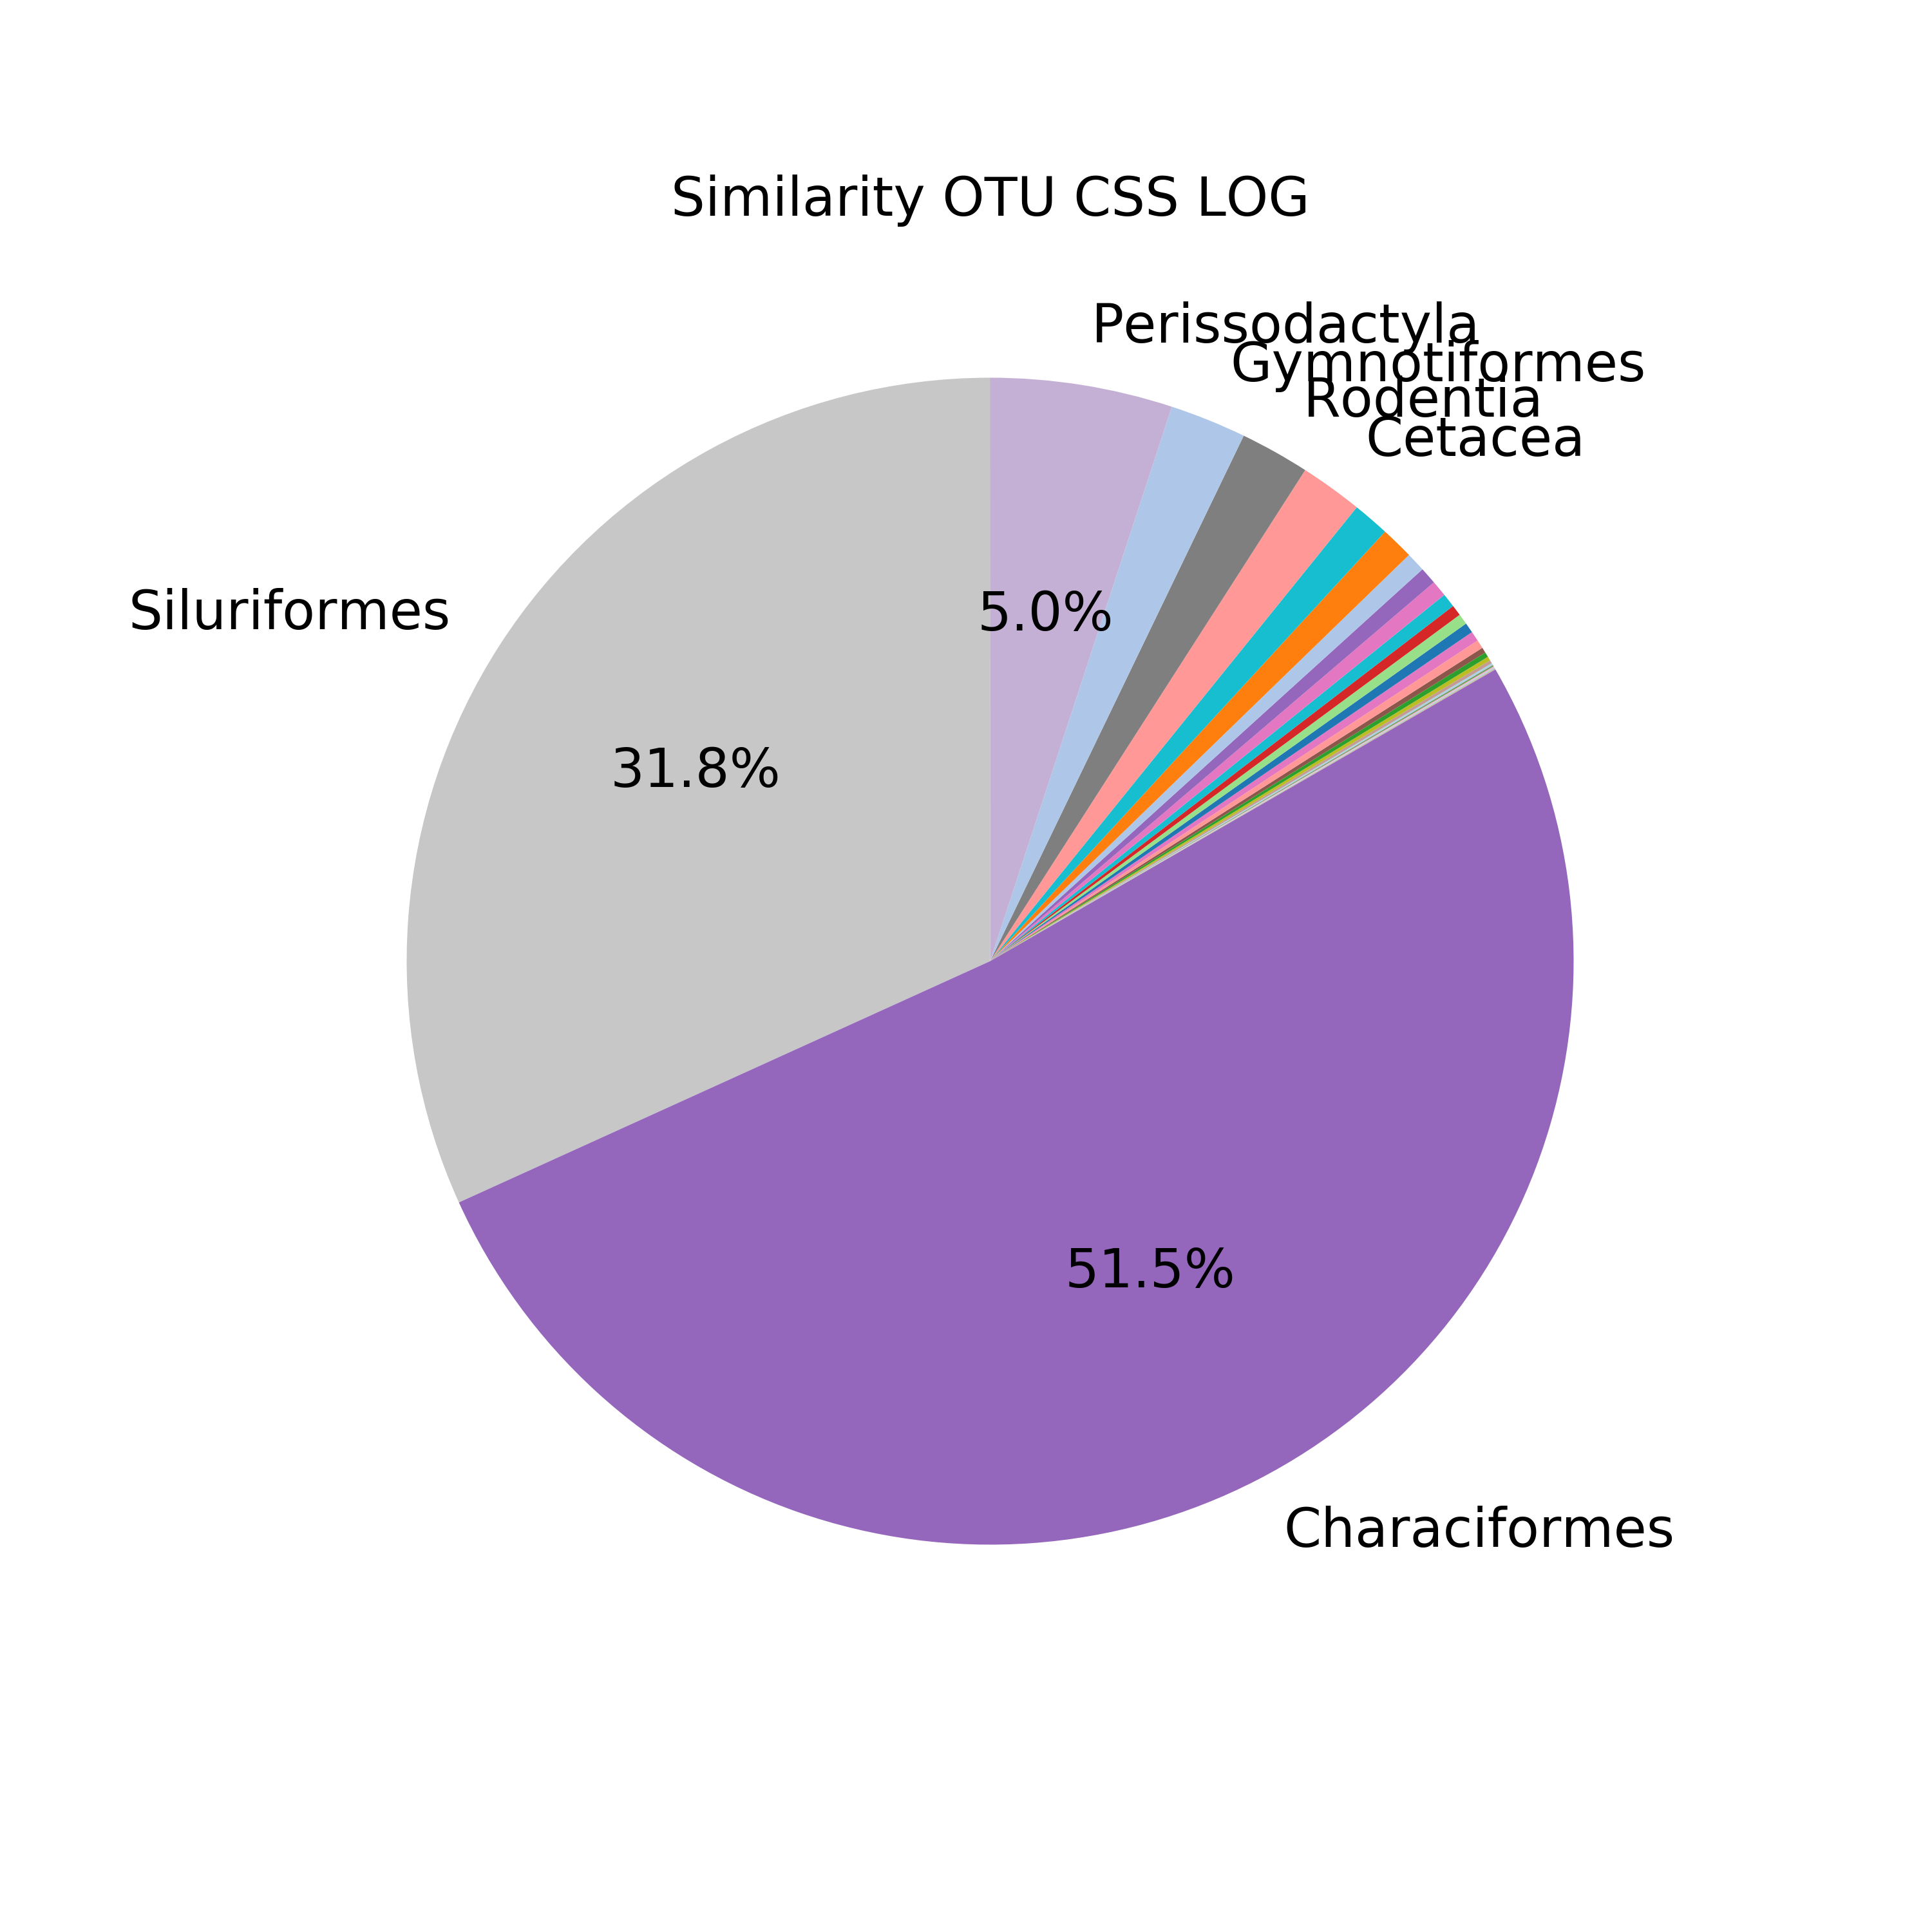
\includegraphics[width=\textwidth]{rfr_sim_sum_pieOTU CSS LOG}
	\caption{}
	\label{fig:simsumotucsslog}
	\end{subfigure}

		\caption{Species' importance per taxonomic order as calculated by Random Forest in the maximum similarity test. Averaging the importance for the sets: OTU CSS \ref{fig:simmeanotucss}, and OTU CSS LOG \ref{fig:simmeanotucsslog}. Summing the importance for the sets: OTU CSS \ref{fig:simsumotucss}, and OTU CSS LOG \ref{fig:simsumotucsslog}. }
	\label{fig:simpie}
\end{figure}

Conclusions can be drawn despite the seemingly contradictory representations of the two methods. This is because all four important Orders are in the top 6 in both methods, and when combined they amount for a substantial part of explanatory power (more than 70\%).    


% DISSIMILARITY
\section{Maximum Dissimilarity}

The classifiers' performance in a maximum dissimilarity setting is worse than that of maximum similarity. The results are summarised in tables \ref{table:lrdissimilarity} and \ref{table:rfrdissimilarity} for Logistic regression and Random Forests respectively. In this setting, Random forests have on average a higher accuracy score. The highest is obtained with OTU MIN CSS (90.45\%), but OTU CSS and OTU CSS LOG come close (90.24\%). Logistic regression has the highest accuracy with PCoA CSS and OTU CSS LOG (87.80\%), and with PCoA coming close (86.58\%). If we consider only some of the axes of PCoA and PCoA CSS, the method attains an even higher accuracy (see table \ref{table:lrdissimilarityappendix} in the Appendix).

Some of the feature sets had an accuracy score close to the baseline, meaning that the classifiers were not significantly better than random guessing. Furthermore, both classifiers had black water Recall scores lower than 0.5 for all of their feature sets, and made a disproportionate amount of errors in classifying these samples. 

Results for PCoA sets explaining 99\% and 90\% of the variance, and for the NMDS configuration, are given in tables \ref{table:lrdissimilarityappendix} and \ref{table:rfrdissimilarityappendix} in the Appendix.

Again, the $L_1$ penalty reduced many coefficients to zero; among the best performing sets,  PCoA CSS had 88.33\% of it's coefficients go to zero, OTU CSS LOG had 95.58\%, and PCoA 90.78\%. The sets OTU, OTU CSS, and OTU CSS LOG shared 3.05\% of their non zero coefficients. This means that once again only a limited number of OTUs contribute to the classification. 
 
% Logistic Dissimilarity
\begin{table}[!h]
	\centering
		\caption{Results from maximising dissimilarity using Logistic Regression}
	\label{table:lrdissimilarity}
	\begin{tabular}{l c  c c}
		\toprule
		&\multicolumn{2}{c}{Confusion Matrix} & Accuracy\\
		Features used & Predicted Black&Predicted White&\\
		\midrule
		\multirow{2}{*}{OTU} &5 &16&\multirow{2}{*}{79.27\%}\\
		&	 18&125&\\
		\cmidrule{2-3}
		\multirow{2}{*}{OTU LOW} &5 &16&\multirow{2}{*}{79.88\%}\\
		&	 17&126&\\
		\cmidrule{2-3}
		\multirow{2}{*}{OTU CSS}&7 &14&\multirow{2}{*}{82.93\%}\\
		&	 14&129&\\
		\cmidrule{2-3}
		\multirow{2}{*}{OTU Min CSS}&3 &18&\multirow{2}{*}{79.61\%}\\
		&	 14&122&\\
		\cmidrule{2-3}
		\multirow{2}{*}{OTU CSS LOG}&5 &16&\multirow{2}{*}{87.80\%}\\
		&	 4&139&\\
		\cmidrule{2-3}
		\multirow{2}{*}{PCoA Bray-Curtis} &7 &14&\multirow{2}{*}{86.59\%}\\
		&	 8&135&\\
		\cmidrule{2-3}
		\multirow{2}{*}{PCoA Bray-Curtis CSS} &9 &12&\multirow{2}{*}{87.80\%}\\
		&	 8&135&\\
		\bottomrule
	\end{tabular}

\end{table}



% RFR dissimilarity table
\begin{table}[!h]
	\centering
		\caption{Results from maximising dissimilarity using Random Forest}
	\label{table:rfrdissimilarity}
	\begin{tabular}{l c  c c}
		\toprule
		&\multicolumn{2}{c}{Confusion Matrix} & Accuracy\\
		Features used & Predicted Black&Predicted White&\\
		\midrule
		\multirow{2}{*}{OTU} &4 &17&\multirow{2}{*}{83.50\%}\\
		&	 10&133&\\
		\cmidrule{2-3}
		\multirow{2}{*}{OTU LOW} &2&19&\multirow{2}{*}{82.32\%}\\
		&	 10&133&\\
		\cmidrule{2-3}
		\multirow{2}{*}{OTU CSS}&7 &14&\multirow{2}{*}{90.24\%}\\
		&	 2&141&\\
		\cmidrule{2-3}
		\multirow{2}{*}{OTU Min CSS}&7 &14&\multirow{2}{*}{90.45\%}\\
		&	 1&135&\\
		\cmidrule{2-3}
		\multirow{2}{*}{OTU CSS LOG}&7 &14&\multirow{2}{*}{90.24\%}\\
		&	 2&141&\\
		\cmidrule{2-3}
		\multirow{2}{*}{PCoA Bray-Curtis} &0 &21&\multirow{2}{*}{86.59\%}\\
		&	 1&142&\\
		\cmidrule{2-3}
		\multirow{2}{*}{PCoA Bray-Curtis CSS} &0 &21&\multirow{2}{*}{84.15\%}\\
		&	 5&138&\\
		\bottomrule
	\end{tabular}

\end{table}

The feature importance method of Random Forest was again employed to explore which species contributed most to their predictive power. Averaging the importance within taxonomic Order for OTU CSS  and OTU CSS LOG is shown in Figures \ref{fig:dissimotucss} and \ref{fig:dissimotucsslog} respectively. For the feature sets OTU and OTU MIN CSS the Figures are \ref{fig:dissimotumean} and \ref{fig:dissimotumincssmean} respectively, presented in the Appendix. As was the case for the maximum similarity setting, \textit{Perissodactyla} is on average the Order with the most explanatory species, with \textit{Cetacea} coming second.


Summing instead of averaging produces the same result seen previously in the maximum similarity setting. Once again \textit{Characiformes} are in sum the most explanatory Order, and \textit{Siluriformes} the second most explanatory. The pie charts for OTU CSS and OTU CSS LOG can be seen in Figures \ref{fig:dissimsumotucss} and \ref{fig:dissimsumotucsslog}, for OTU and OTU MIN CSS in Figures \ref{fig:dissimotusum} and \ref{fig:dissimotumincsssum} in the Appendix. 

The same conclusions are drawn for this setting as well; all four taxonomic Orders are within the six most explanatory ones in both aggregating methods. This suggests that they are indeed useful in prediction,
%%DISIMILARITY PIE CHART
\begin{figure}[!h]
	\centering
	\begin{subfigure}{0.45\textwidth}
		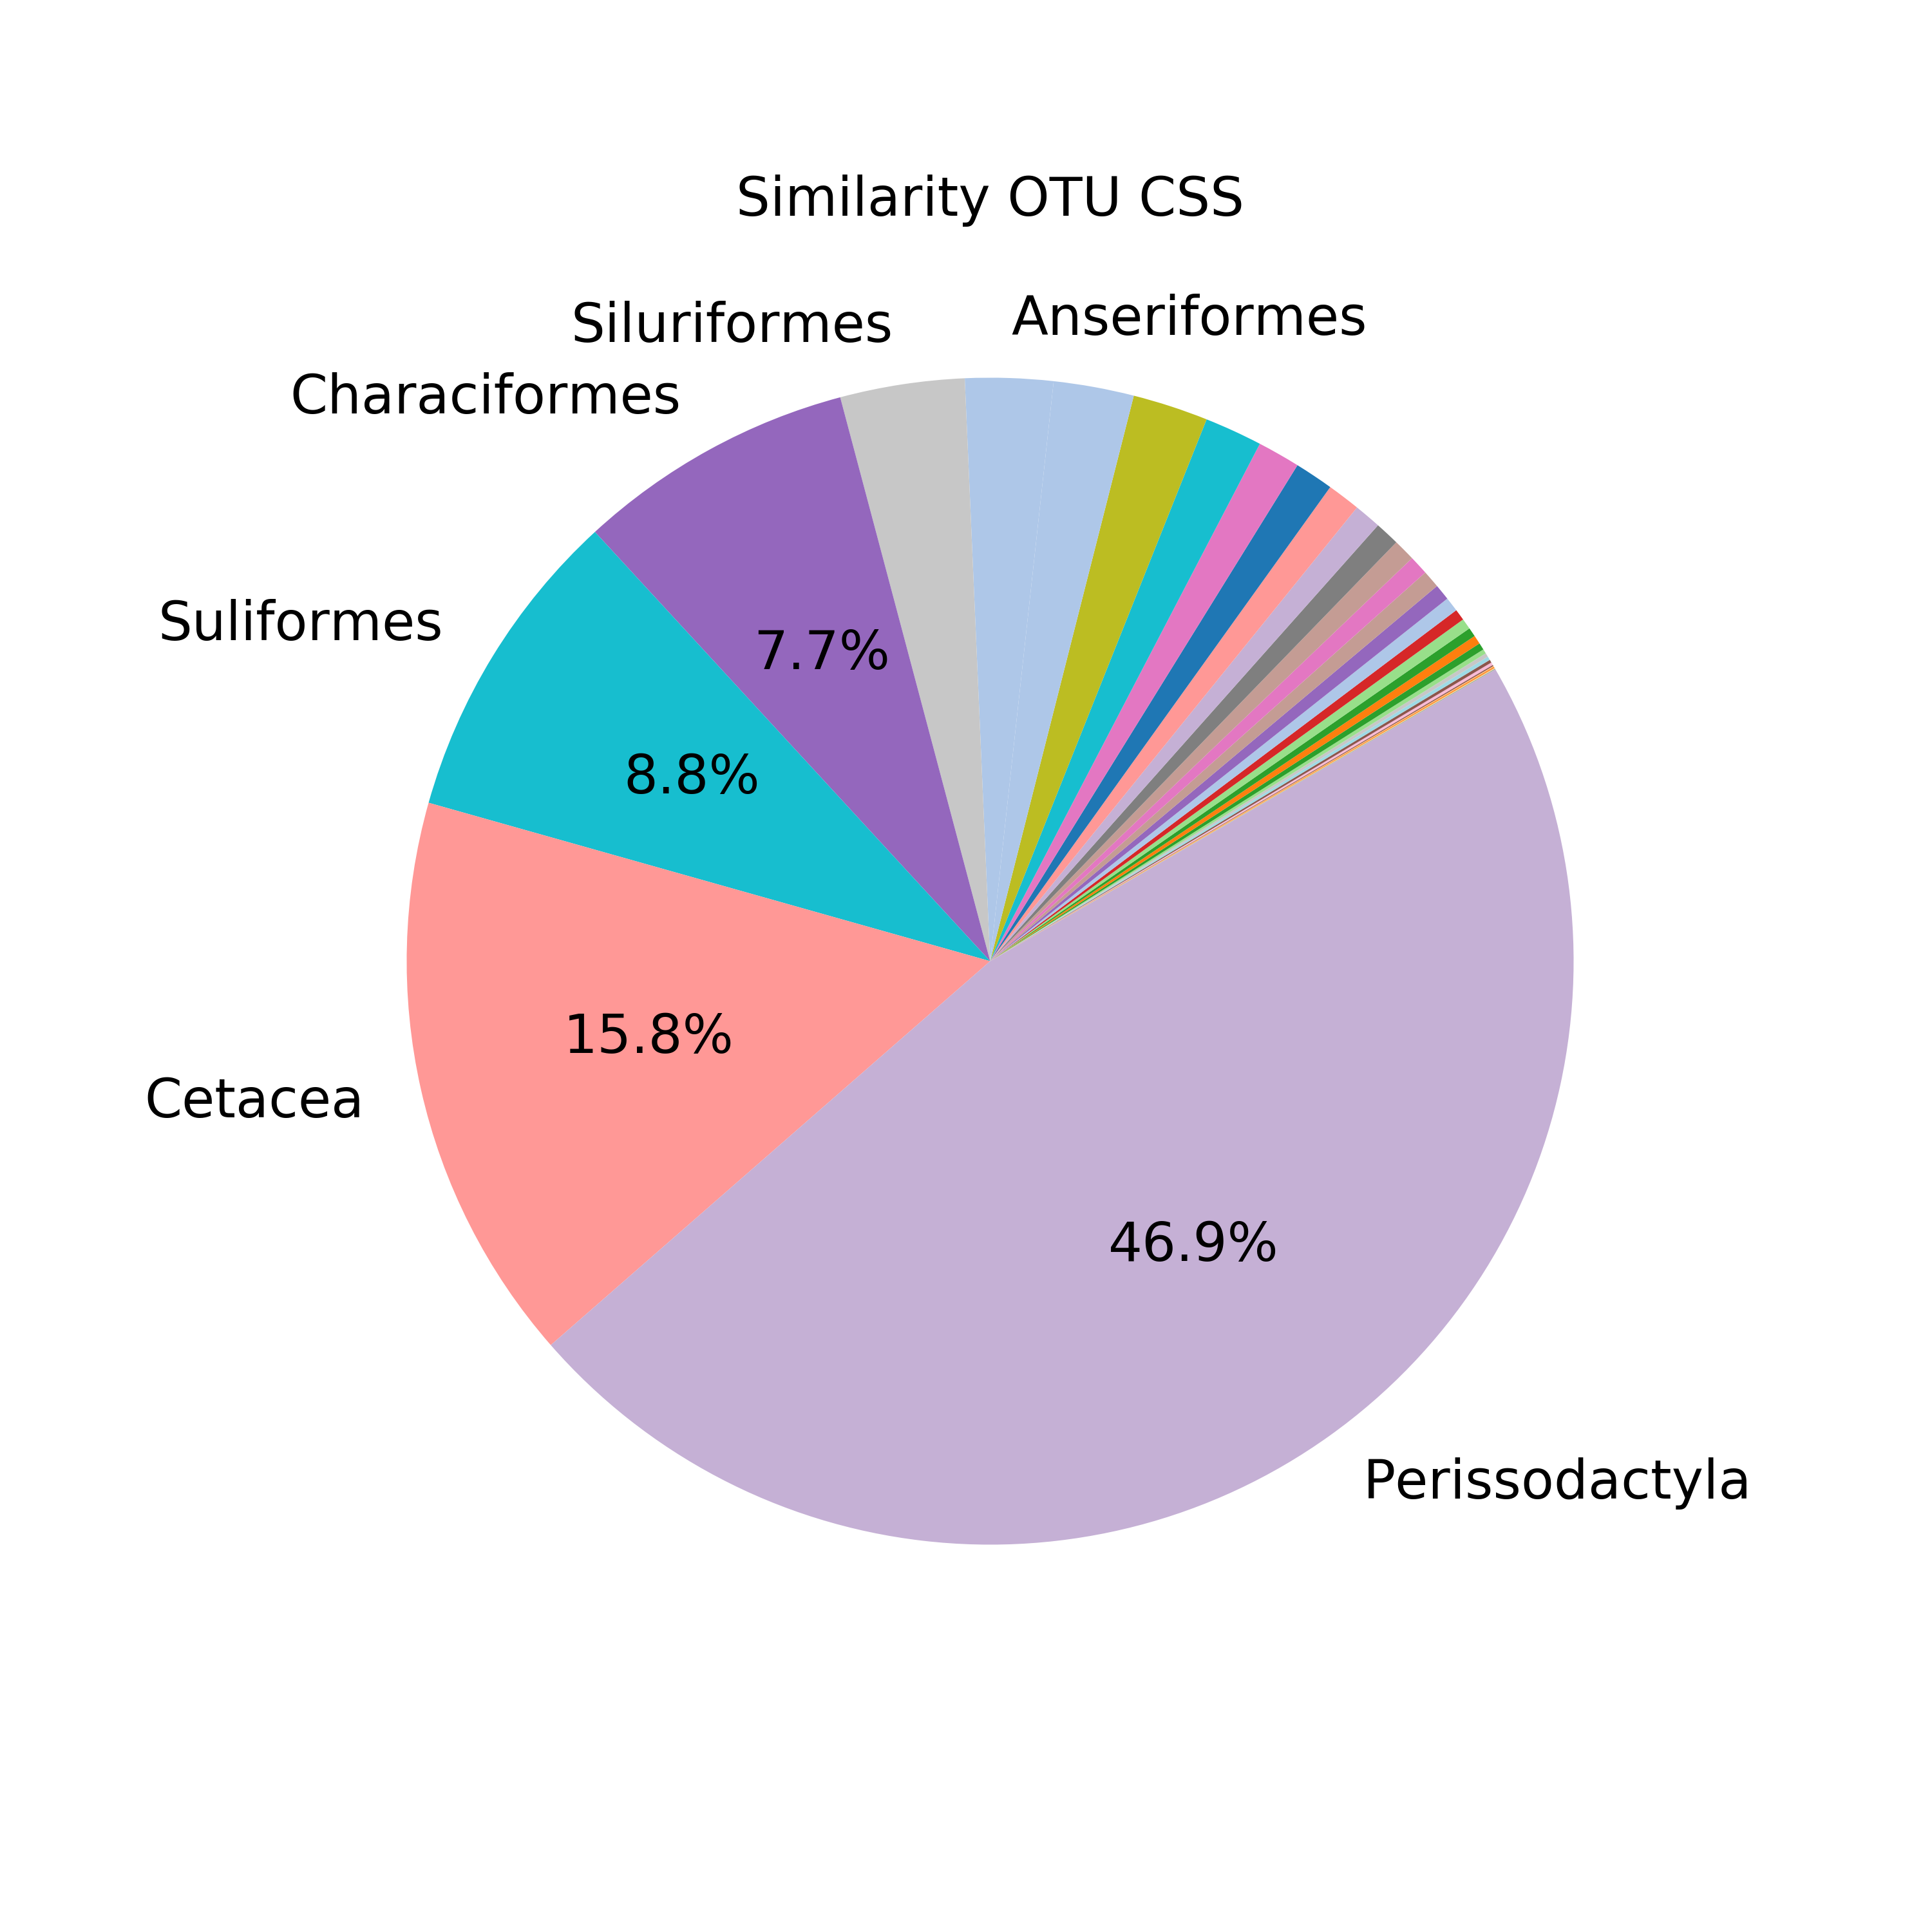
\includegraphics[width=\textwidth]{rfr_dis_mean_pieOTU CSS}
		\caption{}
		\label{fig:dissimotucss}
	\end{subfigure}
	\begin{subfigure}{0.45\textwidth}
		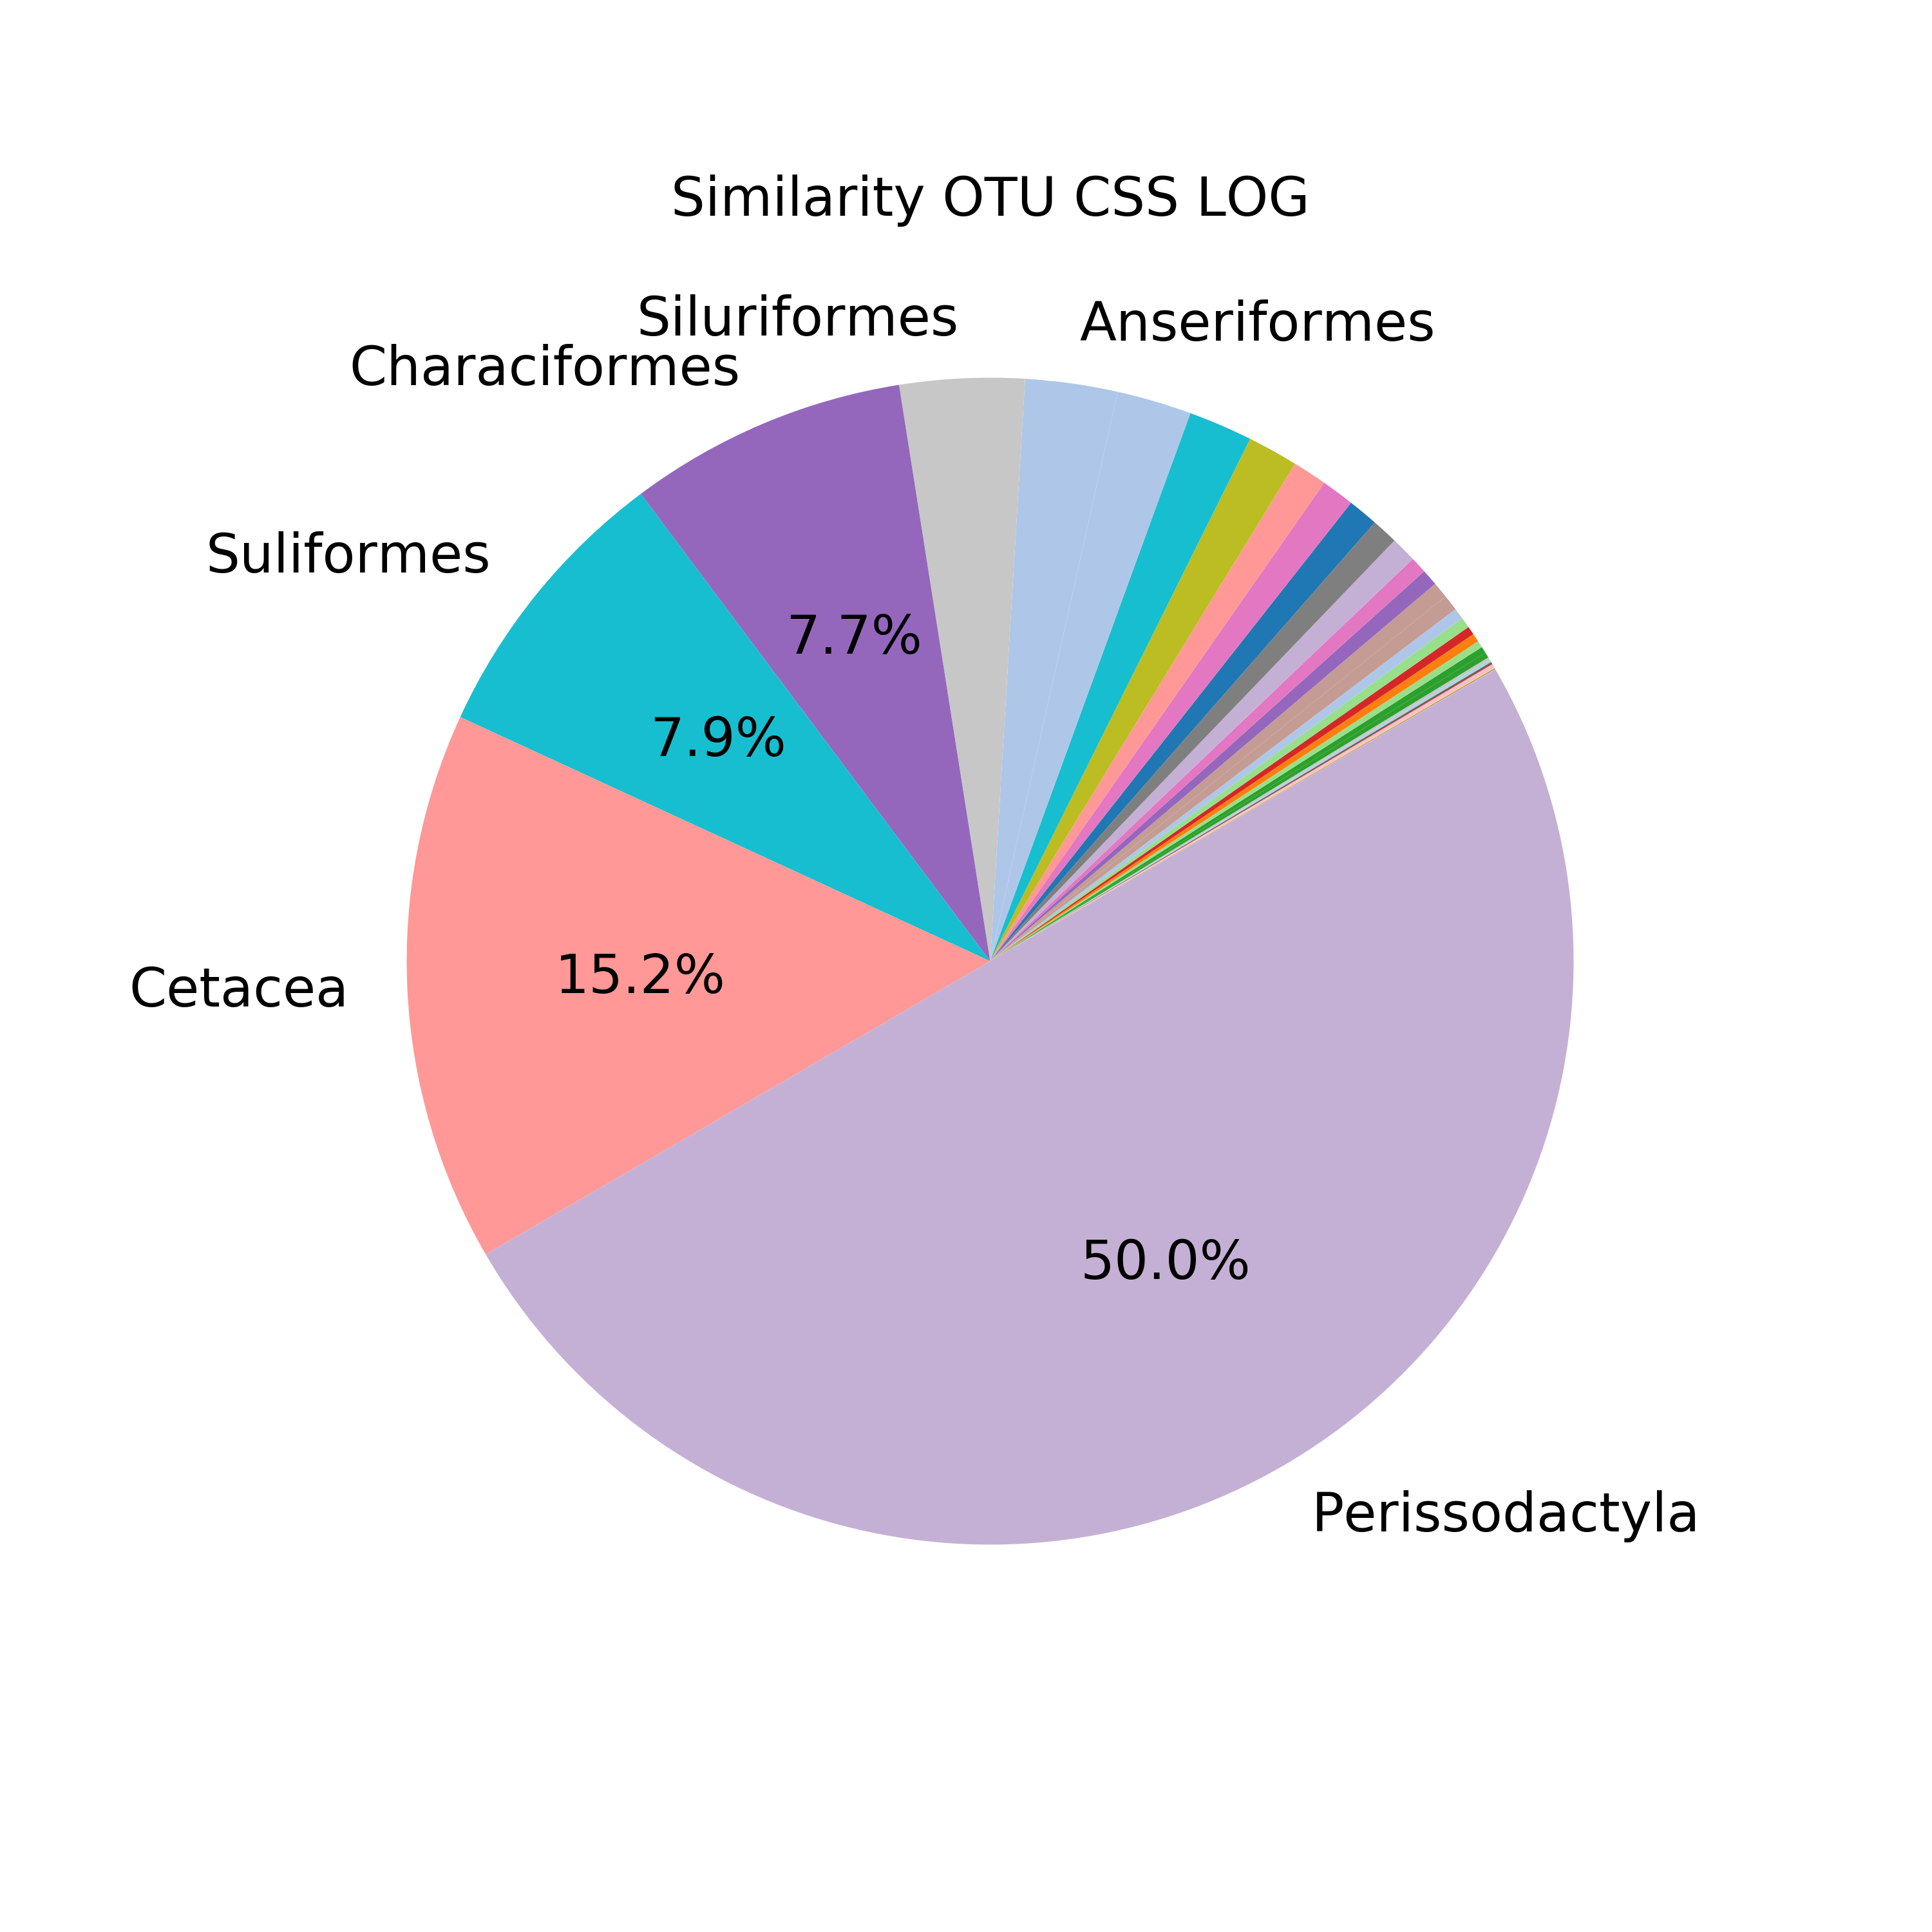
\includegraphics[width=\textwidth]{rfr_dis_mean_pieOTU CSS LOG}
		\caption{}
		\label{fig:dissimotucsslog}
	\end{subfigure}\\
		\begin{subfigure}{0.45\textwidth}
		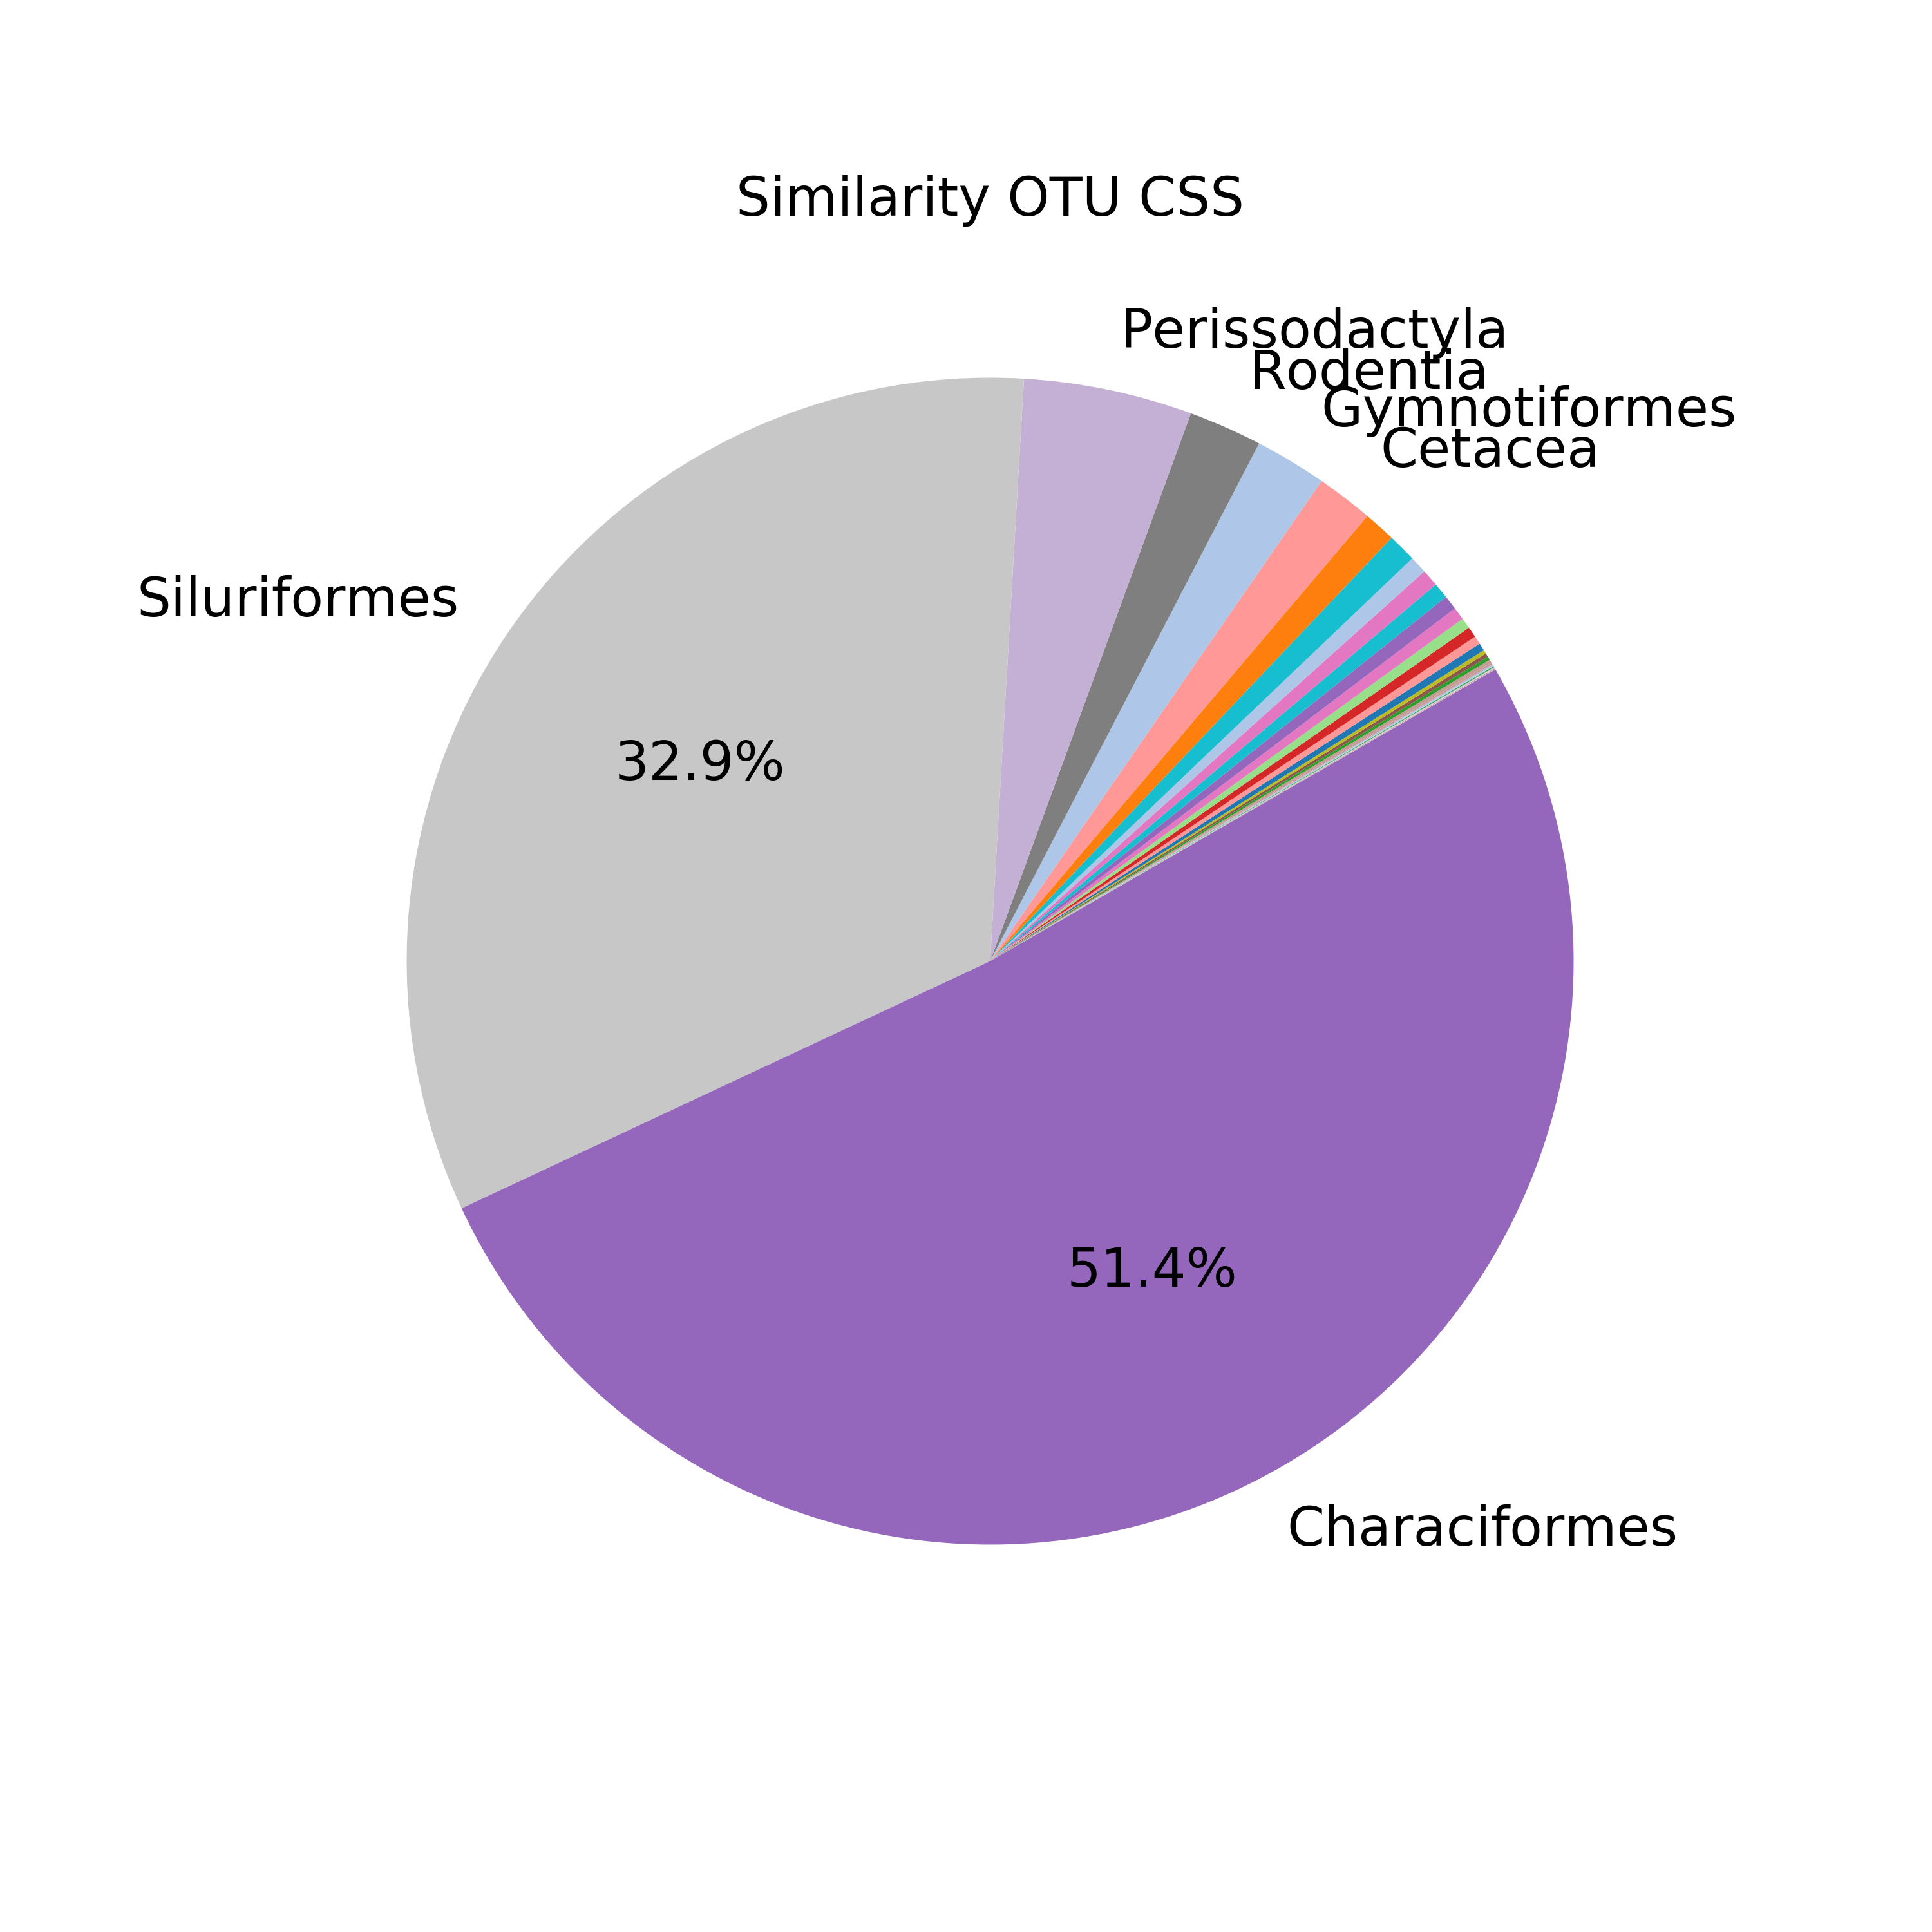
\includegraphics[width=\textwidth]{rfr_dis_sum_pieOTU CSS}
		\caption{}
		\label{fig:dissimsumotucss}
	\end{subfigure}
	\begin{subfigure}{0.45\textwidth}
	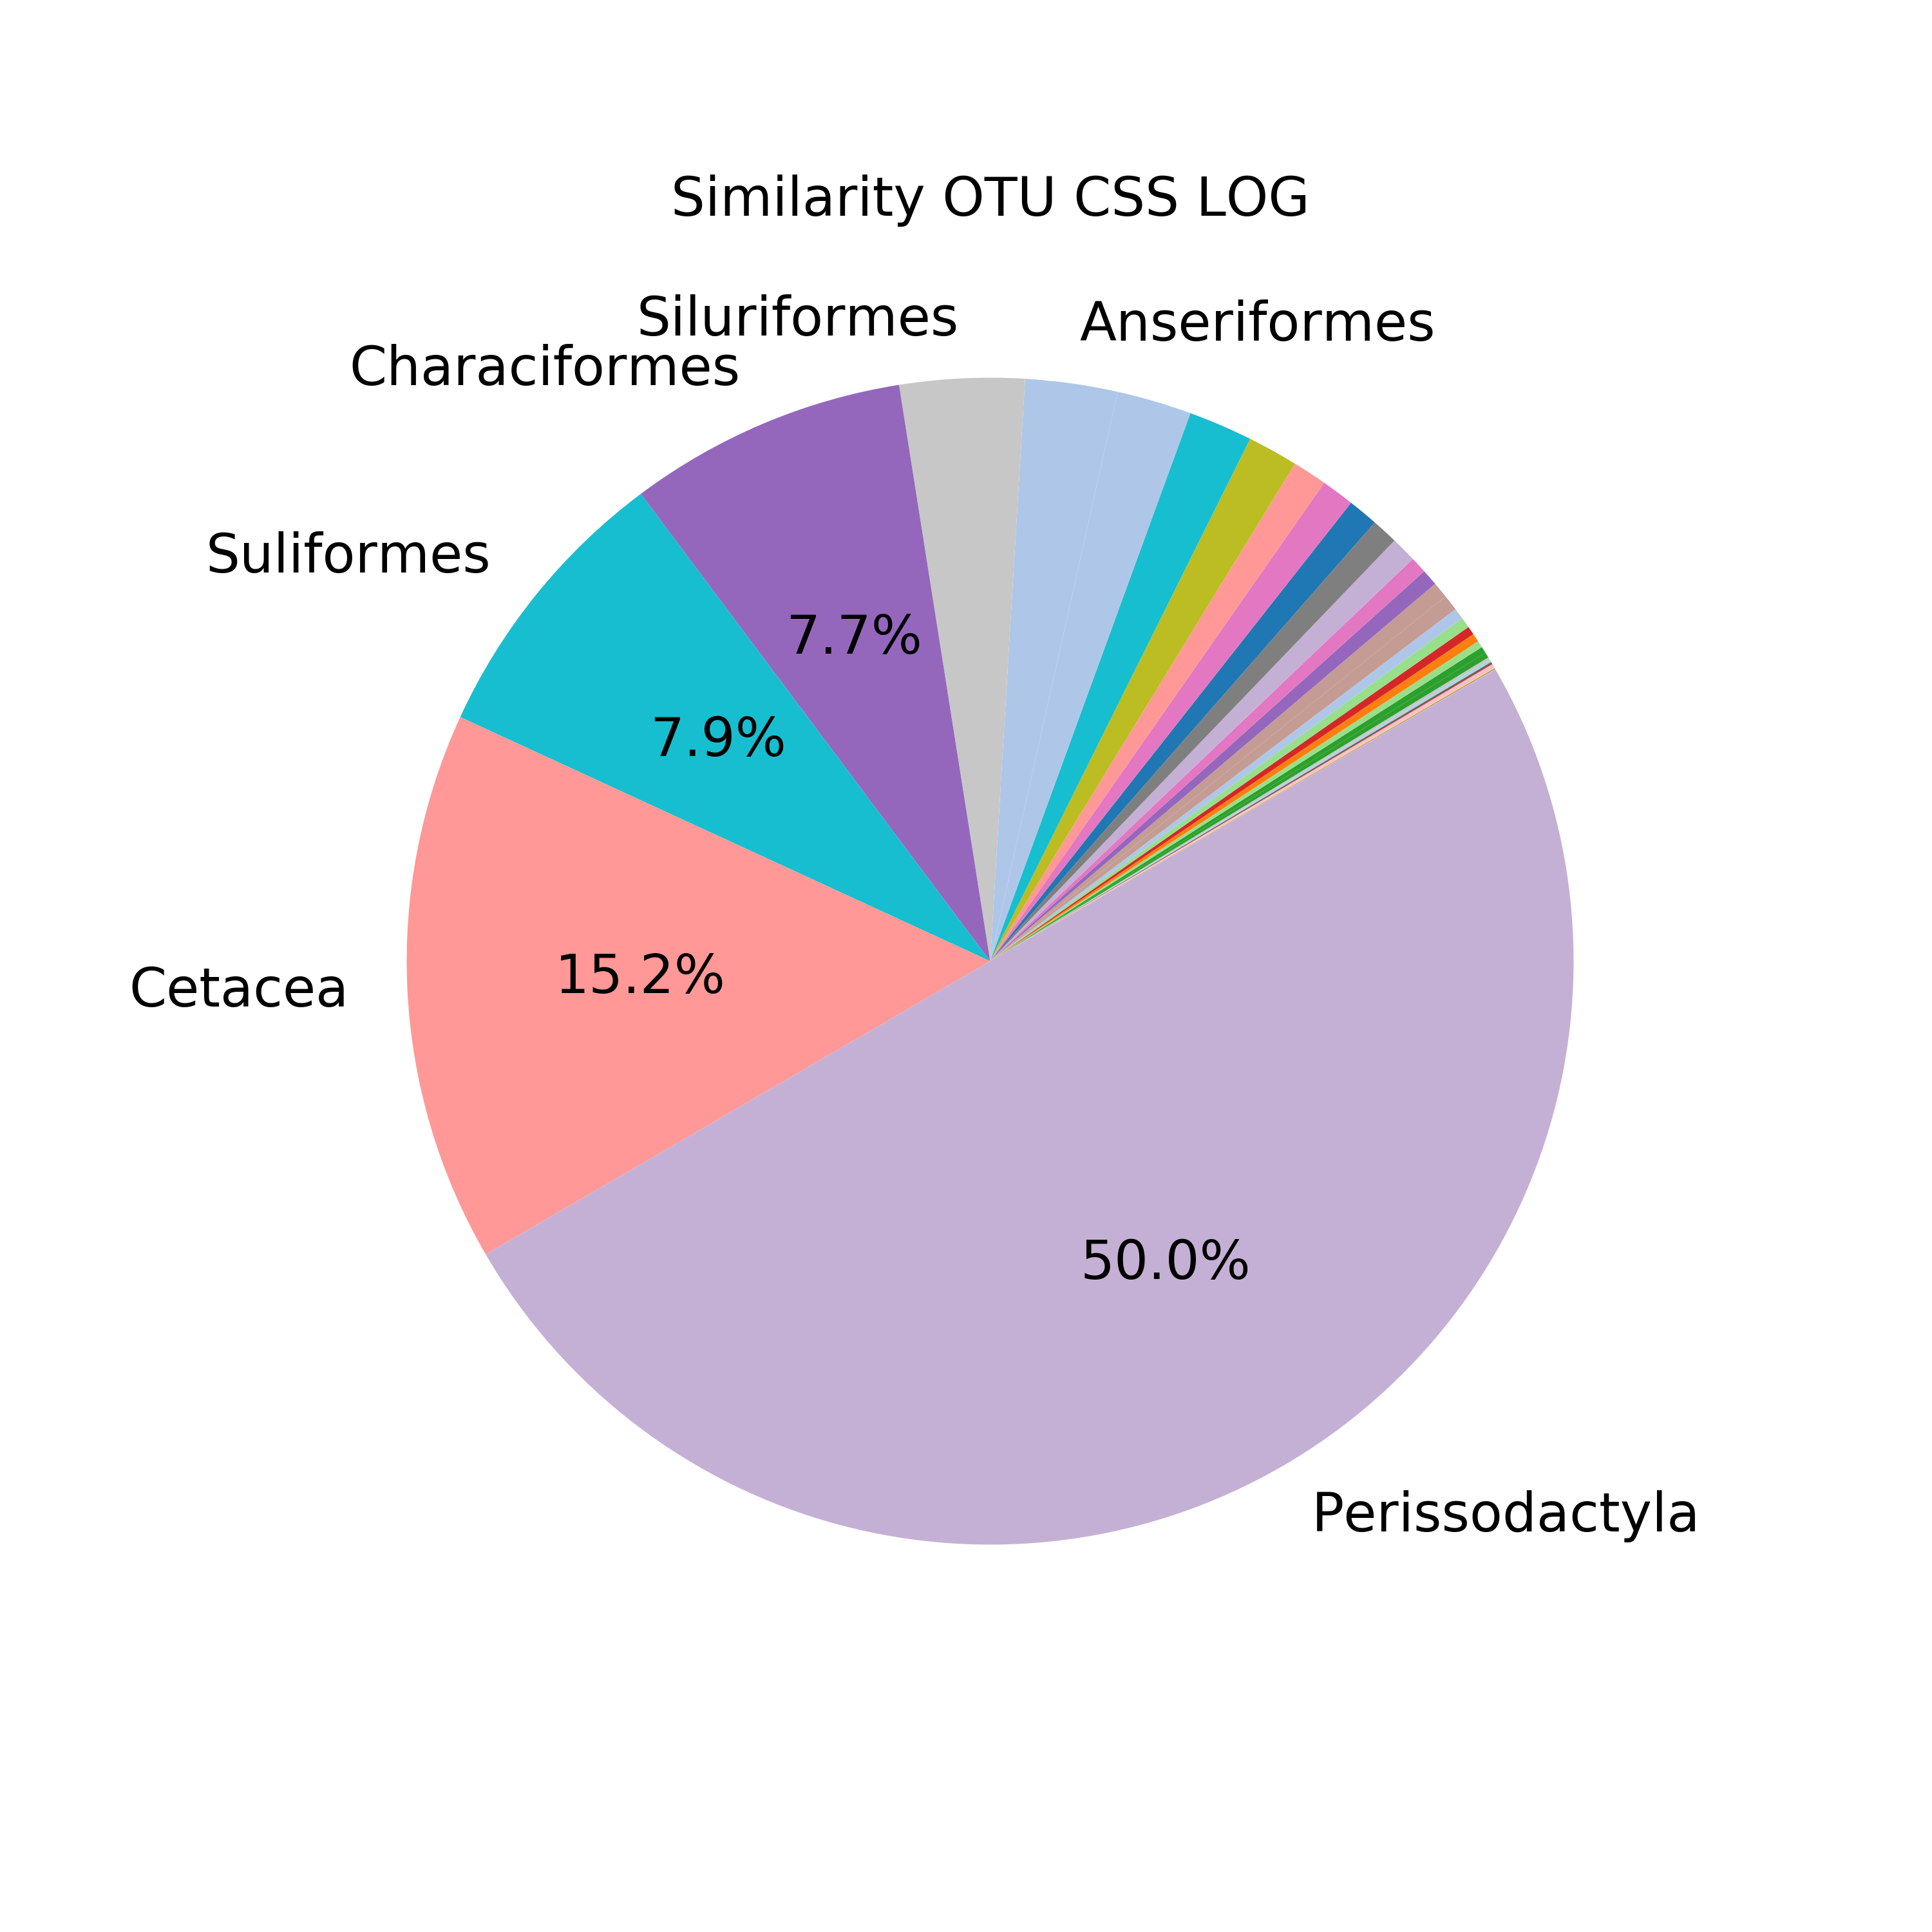
\includegraphics[width=\textwidth]{rfr_dis_sum_pieOTU CSS LOG}
	\caption{}
	\label{fig:dissimsumotucsslog}
\end{subfigure}\\

	\caption{Species' importance per taxonomic order as calculated by Random Forest in the maximum dissimilarity test. Averaging the importance for the sets: OTU CSS \ref{fig:dissimotucss}, and OTU CSS LOG \ref{fig:dissimotucsslog}. Summing the importance for the sets: OTU CSS \ref{fig:dissimsumotucss}, and OTU CSS LOG \ref{fig:dissimsumotucsslog}.
	 }
	\label{fig:dispie}
\end{figure}

\section{Random Splits}
The classifiers' performance under the Random splitting setting is between than of maximum similarity and dissimilarity. The results are summarised in tables \ref{table:lrrandom} for Logistic regression and \ref{table:rfrrandom} for Random Forest. Both methods have accuracy scores significantly better than the baseline.


The best features set for Logistic regression is OTU CSS LOG with 96.34\% accuracy. For Random Forest it is OTU CSS LOG and OTU CSS with a score of 95.73\%. Neither classifier performs better than the other consistently for all features sets. 


Overall, when taking into consideration all the splitting settings, the features set that produces on average the highest accuracy score is OTU CSS LOG. Furthermore, it seems that the sets produced using PCoA fair better when used in Logistic regression, whereas the NMDS configuration is better used by Random Forest (see Appendix).
%LOGISTIC RANDOM
\begin{table}[!h]
	\centering
	\caption{Results from random splits using Logistic Regression}
	\label{table:lrrandom}
	\begin{tabular}{l c  c c}
		\toprule
		&\multicolumn{2}{c}{Confusion Matrix} & Accuracy\\
		Features used & Predicted Black&Predicted White&\\
		\midrule
		\multirow{2}{*}{OTU} &18 &3&\multirow{2}{*}{94.51\%}\\
		&	6&137&\\
		\cmidrule{2-3}
		\multirow{2}{*}{OTU LOW} &17 &4&\multirow{2}{*}{88.41\%}\\
		&	 9&134&\\
		\cmidrule{2-3}
		\multirow{2}{*}{OTU CSS}&16 &5&\multirow{2}{*}{87.20\%}\\
		&	 16&127&\\
		\cmidrule{2-3}
		\multirow{2}{*}{OTU Min CSS}&15 &6&\multirow{2}{*}{82.17\%}\\
		&	 22&114&\\
		\cmidrule{2-3}
		\multirow{2}{*}{OTU CSS LOG}&18 &3&\multirow{2}{*}{96.34\%}\\
		&	6&137&\\
		\cmidrule{2-3}
		\multirow{2}{*}{PCoA Bray-Curtis} &14 &7&\multirow{2}{*}{91.46\%}\\
		&	 7&136&\\
		\cmidrule{2-3}
		\multirow{2}{*}{PCoA Bray-Curtis CSS} &11 &10&\multirow{2}{*}{88.41\%}\\
		&	9&134&\\
		\bottomrule
	\end{tabular}
	
\end{table}

%RFR RANDOM
\begin{table}[!h]
	\centering
	\caption{Results from random splits using Random Forest}
	\label{table:rfrrandom}
	\begin{tabular}{l c  c c}
		\toprule
		&\multicolumn{2}{c}{Confusion Matrix} & Accuracy\\
		Features used & Predicted Black&Predicted White&\\
		\midrule
		\multirow{2}{*}{OTU} &15 &6&\multirow{2}{*}{95.12\%}\\
		&	2&141&\\
		\cmidrule{2-3}
		\multirow{2}{*}{OTU LOW} &15 &6&\multirow{2}{*}{90.24\%}\\
		&	10&143&\\
		\cmidrule{2-3}
		\multirow{2}{*}{OTU CSS}&17 &4&\multirow{2}{*}{95.73\%}\\
		&	 3&140&\\
		\cmidrule{2-3}
		\multirow{2}{*}{OTU Min CSS}&17 &4&\multirow{2}{*}{95.54\%}\\
		&	 3&133&\\
		\cmidrule{2-3}
		\multirow{2}{*}{OTU CSS LOG}&17 &4&\multirow{2}{*}{95.73\%}\\
		&	 3&140&\\
		\cmidrule{2-3}
		\multirow{2}{*}{PCoA Bray-Curtis} &4 &17&\multirow{2}{*}{85.37\%}\\
		&	 7&136&\\
		\cmidrule{2-3}
		\multirow{2}{*}{PCoA Bray-Curtis CSS} &4 &17&\multirow{2}{*}{85.37\%}\\
		&	 2&141&\\
		\bottomrule
	\end{tabular}
	
\end{table}


